% =========================================================================
% CogniLink: IEEE journal article (IEEEtran, journal mode, two columns)
% Device paper: design, implementation, and bench characterization.
% Evaluation with patients, caregivers, and clinicians is planned for a
% separate paper and is deliberately not part of this one.
%
% Compile with pdfLaTeX and BibTeX (Overleaf default).
%
% Conventions used in this draft
%   \tbd{...}   red text: information only the authors can supply
%   \chk{...}   red text: a statement or number in the source material that
%               must be confirmed or corrected before submission
%   \userfig    includes figures/<file> if it exists, otherwise draws a
%               grey placeholder box with a description of the figure
%   \bnimg      places Bengali text pre-rendered with XeLaTeX
%               (snippets/bengali.pdf, source snippets/bengali.tex)
% Remove the \tbd and \chk definitions once every note is resolved; any
% note left behind will then stop compilation and so cannot be missed.
% =========================================================================
\documentclass[journal]{IEEEtran}

\usepackage{cite}
\usepackage{amsmath}
\usepackage{graphicx}
\usepackage{textcomp}
\usepackage{xcolor}
\usepackage{booktabs}
\usepackage{array}
\usepackage{url}
\expandafter\def\expandafter\UrlBreaks\expandafter{\UrlBreaks\do\_}
\usepackage{tikz}
\usetikzlibrary{positioning,arrows.meta,fit,calc}
\usepackage{pgfplots}
\pgfplotsset{compat=1.18}
\usepgfplotslibrary{groupplots}

% ==== Notes for the authors (delete before submission)
\newcommand{\tbd}[1]{\textcolor{red}{[#1]}}
\newcommand{\chk}[1]{\textcolor{red}{[CHECK: #1]}}
\newcommand{\figholder}[2]{%
  \fbox{\parbox[c][#1][c]{0.94\linewidth}{\centering\footnotesize\textcolor{gray}{#2}}}}
% \userfig{file}{includegraphics options}{placeholder height}{placeholder text}
\newcommand{\userfig}[4]{%
  \IfFileExists{#1}{\includegraphics[#2]{#1}}{\figholder{#3}{#4}}}

% ==== Bengali text
% \bnimg[scale]{page} inserts one page of snippets/bengali.pdf on the text
% baseline. Page map: 1 to 8 emergency labels, 9 to 16 spoken sentences
% (same order as Table V), 17 conjunct example, 18 the word "hasanta",
% 19 example conjuncts, 20 the hasanta sign, 21 and 22 the two keyboard
% tab labels.
\newcommand{\bnimg}[2][1]{%
  \raisebox{-#1\dimexpr 3.6pt\relax}{
\includegraphics[scale=#1,page=#2]{snippets/bengali.pdf}}}

% ==== Units
\newcommand{\dps}{\ensuremath{^{\circ}}/s}
\newcommand{\degC}{\ensuremath{^{\circ}}C}

\begin{document}
\bstctlcite{IEEEexample:BSTcontrol}

\title{CogniLink: A Low-Cost Wearable Motion-Tracking Human-Machine Interface and Bilingual Augmentative Communication Dashboard for Severe Motor Impairment}



\markboth{IEEE Journal Name (to be confirmed), Vol.~XX, No.~X, Month~2026}%
{Sadman \MakeLowercase{\textit{et al.}}: CogniLink: Wearable Motion-Tracking Interface and Bilingual AAC Dashboard}

\maketitle

% The abstract was written last, after all other sections.
% Update its numbers if resolving the CHECK notes in Sections VII and VIII
% changes any of them.
\begin{abstract}
People with severe motor impairment often cannot speak or use a standard mouse, and the devices that give them access to augmentative and alternative communication (AAC) are costly and rarely support languages such as Bengali. This paper presents CogniLink, an open-source system that pairs a wearable inertial pointer with a bilingual Bengali and English communicator. A commodity module, worn on a finger or at four other body sites, corrects its gyroscope for bias, applies a velocity control law with threshold subtraction and saturation, and appears to phones, tablets, and computers as a standard Bluetooth Low Energy mouse, so no driver is needed. The same module serves a web communicator with English and Bengali keyboards, the latter ordered by place of articulation and forming conjuncts through the hasanta, together with dwell selection, eight bilingual emergency phrases, and speech with an offline fallback. The hardware costs US\$15. Bench tests with three units and four hosts measured a motion-to-photon latency of $44.35\pm4.36$~ms on a 60~Hz television, which a stage model attributes mainly to the Bluetooth connection interval and the display. With the deadzone enabled, the cursor did not move during 60~s at rest, against $25.4\pm4.2$~px of drift without it. Dwell selections fired $2.41\pm4.13$~ms after their nominal times, offline speech started after 43.6~ms in English and 58.3~ms in Bengali, and the pointer operated two third-party web communicators on Windows, macOS, Android, and Linux. These results set a technical baseline for clinical evaluation.
\end{abstract}

\begin{IEEEkeywords}
Assistive technology, augmentative and alternative communication, Bengali orthography, Bluetooth Low Energy, dwell selection, human-machine interface, inertial measurement unit, microcontroller firmware, motion-to-photon latency, vertical synchronization, wearable sensors.
\end{IEEEkeywords}

% =========================================================================
\section{Introduction}
\label{sec:intro}
% =========================================================================

\IEEEPARstart{P}{eople} who lose speech and most voluntary movement through amyotrophic lateral sclerosis (ALS), cerebral palsy (CP), high cervical spinal cord injury at the C3 to C5 levels, or brainstem stroke often keep the ability to understand others and to decide what they want to say. In ALS, dysarthria is the first or main sign in 25\% to 30\% of patients and affects more than 80\% overall~\cite{tomik2010}. In a Norwegian registry study of 564 children with CP, about one child in five had no verbal speech~\cite{andersen2010}. Augmentative and alternative communication (AAC) can give these people a voice, but only if they can reach the letters or phrases on a screen. Even with direct access through a mouse, touchscreen, or eye tracker, users of text-based AAC typically produce 8 to 10 words per minute, and switch scanning averages about 1.7, while conversational speech runs at 120 to 185~\cite{waller2025}. The access method therefore sets a firm limit on how quickly and how independently a person can communicate.

Access is harder still in low- and middle-income countries. The World Health Organization and UNICEF estimate that more than 2.5~billion people need at least one assistive product and that access ranges from 3\% in some countries to 90\% in others~\cite{who2022}. In a household survey in two districts of Bangladesh, 71\% of people with a functional difficulty reported an unmet need for assistive products~\cite{pryor2018}. Dedicated head mice and eye trackers cost from about US\$600 to more than US\$1,200 (Table~\ref{tab:comparison}), before the computer that runs the communication software. Language is a second barrier, because work on AAC in languages other than English remains limited~\cite{amery2022}, even for languages with very large populations. Bengali, for example, has about 273~million speakers and ranks seventh among the world's languages by total number of speakers~\cite{britannica}. For a Bengali-speaking family, a usable system has to be affordable, run on devices the family already owns, speak their language, and be repairable with parts that can be bought locally.

Several of the necessary pieces already exist. Wearable head mice translate head rotation into cursor movement~\cite{montechquha,glassouse}, open-source alternative mice present themselves to the host as standard input devices~\cite{lipsync,flipmouse}, and free web communicators offer multilingual boards and hover selection~\cite{cboard,astericsgrid}. What is still missing is a low-cost wearable pointer that needs no driver, paired with a Bengali communicator built around dwell selection and urgent needs, and characterized in enough technical detail that clinicians and engineers can judge whether it is ready for testing with patients.

This paper presents CogniLink, a communication system built from one commodity module and a web application. A unit worn on a finger, or on the wrist, an eyeglass temple, a headband, or the big toe (Fig.~\ref{fig:mounting}), reads angular velocity from its inertial measurement unit (IMU) and moves the cursor of a phone, tablet, or computer, which recognizes it as an ordinary Bluetooth Low Energy (BLE) mouse. The same unit serves the communicator as a web page over Wi-Fi, so the host needs nothing more than a browser. The communicator provides an English keyboard, a Bengali keyboard that follows the traditional order of the alphabet, dwell selection with four dwell times, eight bilingual emergency phrases, and speech output with an offline fallback. The hardware costs US\$15.

% ==== Figure 1: mounting configurations (authors' image) ==================
% ALT TEXT: The CogniLink unit worn as a ring on the index finger, on a wrist
% strap, clipped to an eyeglass temple, in a headband, and on the big toe.
\begin{figure}[!t]
\centering
\userfig{figures/fig1_wearable_mounting.png}{width=\linewidth}{5.0cm}{FIGURE FILE figures/fig1\_wearable\_mounting.png\\[2pt] The unit worn as a ring on the proximal phalanx, on a wrist strap, on an eyeglass temple, in a headband, and on the big toe.}
\caption{Mounting configurations supported by the CogniLink cradle: a dorsal finger ring on the proximal phalanx (default), a wrist strap, an eyeglass temple, a headband, and the dorsum of the big toe (hallux).}
\label{fig:mounting}
\end{figure}

This paper reports the design, implementation, and bench characterization of the system. Evaluation with patients, caregivers, and clinicians is the next stage of the project and will be reported separately. The paper makes four contributions:
\begin{enumerate}
\item A driver-free wearable inertial pointer built on a single commodity module, with a velocity control law that combines bias correction, threshold subtraction, and saturation, and an analysis of its onset, gain, and saturation (Sections~\ref{sec:hardware} and~\ref{sec:firmware}).
\item A bilingual communicator served by the wearable itself, with a Bengali keyboard that forms conjuncts through the hasanta, dwell selection, and a tray of emergency phrases (Section~\ref{sec:communicator}).
\item A bench characterization on four host platforms covering motion-to-photon latency, with a stage-by-stage latency model, resting stability, report timing, dwell timing, power consumption, speech onset, and compatibility with third-party web AAC (Sections~\ref{sec:method} and~\ref{sec:results}).
\item An open release of the hardware design, firmware, communicator, and benchmark data~\tbd{repository URL}.
\end{enumerate}

Section~\ref{sec:related} reviews related work, and Section~\ref{sec:goals} states the design goals. Sections~\ref{sec:hardware} to~\ref{sec:communicator} describe the hardware, firmware, and communicator. Sections~\ref{sec:method} and~\ref{sec:results} present the evaluation methods and results, Section~\ref{sec:discussion} discusses their implications and the limitations of the system, and Section~\ref{sec:conclusion} concludes.

% =========================================================================
\section{Related Work}
\label{sec:related}
% =========================================================================

\subsection{AAC and Access Methods}
High-tech AAC pairs a selection interface with speech output, and the access method largely sets the pace of communication. Direct selection is faster than switch scanning, but both are far slower than speech~\cite{waller2025}. Eye trackers such as the PCEye~5 give gaze-only control of a Windows computer at an estimated cost of US\$1,249~\cite{montechpceye}. Web-based AAC has lowered the software barrier. Cboard, an open-source communication board, lists Bengali among its languages and can run and speak offline in Chrome~\cite{cboard}, and AsTeRICS Grid, a free grid communicator, accepts touch, click, hover, and scanning input and keeps working offline once loaded~\cite{astericsgrid}. These tools solve much of the software problem, but they assume that the user already has a reliable way to point or to press a switch.

\subsection{Motion-Based and Wearable Pointing}
When hand function is limited, cursor control is often moved to the head or face. Camera Mouse tracks a facial feature through a webcam~\cite{betke2002} and is free to use~\cite{vojtech2020}. In an ISO 9241-9 evaluation it reached 0.65~bits/s with dwell selection, against 2.30~bits/s for a touchpad with tapping, and cursor control was erratic, with frequent target re-entries~\cite{hassan2019}. Head tracking with a tablet's front camera reached 1.42~bits/s on the multi-directional task of ISO 9241-411~\cite{roigmaimo2018}. Cameras also depend on lighting and on where the user sits~\cite{kabir2026}. Vojtech et al.\ combined head-tilt accelerometry with facial surface electromyography (EMG); with 24 non-disabled adults this gave better accuracy and path efficiency than Camera Mouse, which was faster~\cite{vojtech2020}, and Groll et al.\ compared click methods for the same kind of accelerometer-based cursor~\cite{groll2020}. Auxilio, developed in Bangladesh, uses a head-mounted IMU to point and infrared sensing of cheek twitches to click, and it communicates with the computer through a receiver and driver software. With 10 participants without motor impairments it scored 78.75 on the System Usability Scale, against 48.75 for a commercial camera-based mouse~\cite{kabir2026}, and its acceptability has been studied with people with upper-limb disability~\cite{kabir2023}. Commercial wearable head mice such as the Quha Zono~\cite{montechquha} and the gyroscopic GlassOuse~\cite{glassouse} follow the same principle at prices of several hundred US dollars or more. Among open designs, LipSync is a mouth-operated joystick with sip-and-puff clicking~\cite{lipsync}, and FLipMouse behaves as a standard mouse, keyboard, or joystick without extra software~\cite{flipmouse}.

Finger-worn IMUs have received less attention as accessibility inputs. MouseRing tracks a finger sliding on a physical surface with one or two IMU rings and came close to touchpad speed in a Fitts' law study with 12 participants~\cite{shen2024}, but it needs a surface and deliberate finger sliding. Mouse on a Ring instead maps the tilt and acceleration of a ring moved in the air to cursor motion~\cite{zhao2021}. We are not aware of a finger-worn in-air pointer that has been combined with dwell-based AAC or with Bengali.

% ==== Table I =============================================================
\begin{table*}[!t]
\caption{CogniLink Compared With Existing Access Devices and AAC Software. Costs Are Published Estimates in US Dollars; n/a Means Not Applicable and n/r Means Not Reported.}
\label{tab:comparison}
\centering
\footnotesize
\begin{tabular}{@{}llllccr@{}}
\toprule
Solution & Type & Input & Selection & Open & Bengali & Cost (USD) \\
\midrule
PCEye 5~\cite{montechpceye} & Eye tracker & Eye gaze & Gaze software & No & n/a & 1,249 \\
Quha Zono~\cite{montechquha} & Head mouse & Head or other body site & Dwell software or switch & No & n/a & 999 \\
GlassOuse v1.4~\cite{glassouse} & Gyroscopic mouse & Head & 0.5\,s dwell or switch & No & n/a & 599 \\
Camera Mouse~\cite{betke2002,vojtech2020} & Camera pointer & Face via webcam & Dwell & n/r & n/a & Free \\
LipSync~\cite{lipsync} & Mouth joystick & Mouth & Sip and puff & Yes & n/a & Under 300 (build) \\
FLipMouse~\cite{flipmouse} & Joystick & Lips or finger & Sip, puff, or switch & Yes & n/a & n/r \\
Cboard~\cite{cboard} & Web AAC & Touch or pointer & Click or touch & Yes & Yes & Free (paid tier) \\
AsTeRICS Grid~\cite{astericsgrid} & Web AAC & Touch, pointer, or switch & Click, hover, or scan & Yes & n/r & Free \\
\midrule
CogniLink (this work) & Pointer and web AAC & Finger, wrist, head, or toe & Dwell or button & Yes & Yes & 15 \\
\bottomrule
\end{tabular}
\end{table*}

\subsection{Dwell Selection}
Dwell selection lets a person click by holding the pointer still. It removes the need for a switch but invites unintended selections whenever the pointer rests on a target, the so-called Midas touch problem~\cite{jacob1990}. Most eye-typing studies have used constant dwell times of 450 to 1000~ms and report 5 to 10 words per minute~\cite{majaranta2009}. Helmert et al.\ obtained their best overall gaze-typing performance with a 500~ms dwell~\cite{helmert2008}, and novices who were allowed to adjust the dwell shortened it from 876 to 282~ms over ten sessions while their speed rose from 6.9 to 19.9 words per minute~\cite{majaranta2009}. Dynamic schemes shorten the dwell for likely keys. Cascading dwell reached 12.39 words per minute against 10.62 for a static dwell with 17 non-disabled participants, and 9.51 words per minute with five people with ALS~\cite{mott2017}. A recent meta-analysis reports 500 to 600~ms as a common balance between speed and accuracy in eye tracking~\cite{burnham2025}. For motion-based pointing the evidence is thinner: Groll et al.\ tested dwell times of 0.5, 1.0, and 1.5~s with a head-tilt accelerometer cursor~\cite{groll2020}. Gaze reaches a target almost at once, whereas a body-worn pointer has to be steered onto it, so dwell times from eye typing may not transfer directly.

\subsection{Text Entry Rate and Word Prediction}
Word and phrase prediction is the most common way to raise AAC text entry rates~\cite{waller2025}, but its benefit depends on the user. Koester and Levine first modeled and then measured this trade-off. The time needed to read and judge a prediction list can offset the keystrokes it saves~\cite{koester1994}, and for users with spinal cord injury, word prediction significantly lowered the text entry rate, while it raised the rate only modestly for able-bodied users~\cite{koester1996}. For a new language and a new input device, these findings argue for measuring the cost of prediction rather than assuming a gain.

\subsection{Bengali Text Entry and Multilingual AAC}
Bengali is written in an abugida. Each consonant carries an inherent vowel, dependent vowel signs (\textit{kar}) attach to consonants, and consonant clusters are written as conjuncts by placing the hasanta (virama, U+09CD) between consonants, which the text renderer then joins into one glyph. One visible character can therefore take several key selections, and the same text can be entered in different ways. Sarcar et al.\ showed that text entry metrics designed for English do not transfer directly to Bengali for this reason and proposed Bengali-specific definitions~\cite{sarcar2015}, and Arif and Fardeen built a phrase set for Bengali text entry evaluations from real text messages~\cite{arif2016}. Among the communicators reviewed above, Cboard supports Bengali~\cite{cboard}, but we are not aware of a Bengali keyboard designed for dwell selection with a body-worn pointer.

% =========================================================================
\section{Design Goals}
\label{sec:goals}
% =========================================================================

From the work reviewed above and the conditions CogniLink is meant for, we set six design goals.

\begin{IEEEdescription}[\IEEEsetlabelwidth{G6}]
\item[G1] \textit{Use whatever movement remains.} Controllable movement differs between people and may decline over time, so the unit can be worn on a finger, wrist, eyeglass temple, headband, or toe, and the dwell time is chosen per user.
\item[G2] \textit{Run on devices people already own.} The pointer should work with phones, tablets, and computers, including computers that drive a television at the bedside, without drivers or apps, as standard input devices such as FLipMouse already do~\cite{flipmouse}. The communicator should need only a browser.
\item[G3] \textit{Speak Bengali and English.} Both languages should be available for typing and for speech, since AAC outside English remains scarce~\cite{amery2022}, and speech should keep working without an internet connection.
\item[G4] \textit{Put urgent needs first.} Requests about suction, pain, breathing, or repositioning should be one selection away, because composing text letter by letter is slow~\cite{waller2025}.
\item[G5] \textit{Keep cost and repair within local means.} The hardware should use commodity parts and an open design, given how limited access to assistive products is in low-resource settings~\cite{who2022,pryor2018}.
\item[G6] \textit{Tolerate drift and small involuntary movement.} Sensor drift and small unintended movements should neither move the cursor nor trigger selections, a known weakness of dwell-based pointing~\cite{jacob1990,hassan2019}.
\end{IEEEdescription}

% =========================================================================
\section{Hardware}
\label{sec:hardware}
% =========================================================================

\subsection{System Overview}
Fig.~\ref{fig:architecture} shows the architecture. The wearable unit maintains two independent links. Over BLE it acts as a standard mouse: gyroscope readings are corrected for bias, passed through a deadzone and a gain, clipped to the range of a mouse report, and sent to the host, whose operating system moves the cursor. Over Wi-Fi it serves the communicator as a single web page and pushes telemetry, including the battery level, to that page. The communicator runs in the host's browser, where it handles dwell selection, message composition, and speech. Because the pointer is an ordinary mouse, it is not tied to the communicator and can also operate other software, including third-party AAC.

% ==== Figure 2: system architecture (TikZ, no image file needed) ==========
% ALT TEXT: Block diagram. In the wearable unit, core 1 runs the gyroscope,
% bias correction, deadzone and gain, and BLE HID mouse blocks; core 0 runs
% the HTTP and WebSocket servers, fed by a battery gauge and reached over
% Wi-Fi in station or setup mode. On the host, BLE reports move the operating
% system cursor, which drives the browser communicator, which produces speech.
\begin{figure}[!t]
\centering
\resizebox{\linewidth}{!}{%
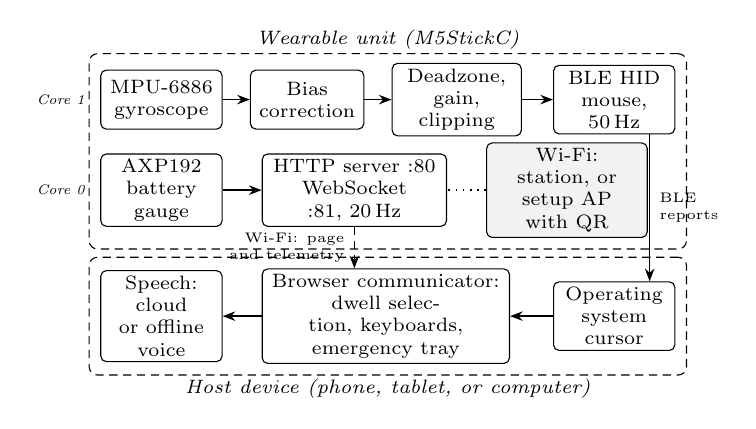
\begin{tikzpicture}[
  font=\scriptsize,
  blk/.style={draw, rounded corners=2pt, align=center, minimum height=7.5mm, inner sep=2pt},
  arr/.style={-{Stealth[length=1.6mm]}, semithick},
  grp/.style={draw, densely dashed, rounded corners=3pt, inner sep=4pt}]
\node[blk, text width=14mm] (imu) at (0,0) {MPU-6886\\gyroscope};
\node[blk, text width=13mm] (cal) at (1.85,0) {Bias\\correction};
\node[blk, text width=15mm] (dz)  at (3.75,0) {Deadzone, gain,\\clipping};
\node[blk, text width=14mm] (hid) at (5.75,0) {BLE HID\\mouse, 50\,Hz};
\node[blk, text width=14mm] (bat) at (0,-1.15) {AXP192\\battery gauge};
\node[blk, text width=22mm] (ws)  at (2.45,-1.15) {HTTP server :80\\WebSocket :81, 20\,Hz};
\node[blk, text width=19mm, fill=gray!10] (qr) at (5.15,-1.15) {Wi-Fi: station, or\\setup AP with QR};
\node[blk, text width=14mm] (tts) at (0,-2.75) {Speech: cloud\\or offline voice};
\node[blk, text width=30mm] (com) at (2.85,-2.75) {Browser communicator:\\dwell selection, keyboards,\\emergency tray};
\node[blk, text width=14mm] (cur) at (5.75,-2.75) {Operating\\system cursor};
\node[font=\tiny\itshape, anchor=east] at (-0.85,0) {Core 1};
\node[font=\tiny\itshape, anchor=east] at (-0.85,-1.15) {Core 0};
\draw[arr] (imu) -- (cal);
\draw[arr] (cal) -- (dz);
\draw[arr] (dz) -- (hid);
\draw[arr] (bat) -- (ws);
\draw[semithick, dotted] (qr) -- (ws);
\draw[arr] (hid.south) ++(0.45,0) -- node[right, font=\tiny, align=left] {BLE\\reports} ($(cur.north)+(0.45,0)$);
\draw[arr] (cur) -- (com);
\draw[arr] (com) -- (tts);
\draw[arr, densely dashed] (ws.south) -- node[left, font=\tiny, align=right] {Wi-Fi: page\\and telemetry} (ws.south |- com.north);
\node[grp, fit=(imu)(hid)(bat)(qr), label={[font=\scriptsize\itshape, inner sep=1pt]above:Wearable unit (M5StickC)}] {};
\node[grp, fit=(tts)(com)(cur), label={[font=\scriptsize\itshape, inner sep=1pt]below:Host device (phone, tablet, or computer)}] {};
\end{tikzpicture}}
\caption{System architecture. On core~1, gyroscope readings are corrected for bias, passed through the deadzone and gain, clipped, and sent to the host as BLE HID mouse reports. On core~0, the unit serves the communicator page and pushes telemetry over Wi-Fi, either through a local network or through its own setup access point. The communicator in the host browser handles dwell selection and speech.}
\label{fig:architecture}
\end{figure}

\subsection{Form Factor and Mounting Sites}
\label{sec:mounting}
The default configuration is a ring module seated on the dorsal side of the proximal phalanx of the dominant index or middle finger (Fig.~\ref{fig:mounting}). An M5StickC module~\cite{m5stickc} sits in a cradle printed in-house by fused deposition modeling (FDM) from polyethylene terephthalate glycol (PETG) and is held by a silicone strap with an adjustable hook-and-loop fastener. The module measures $48.2\times25.5\times13.7$~mm and weighs 15.1~g including its battery~\cite{m5stickc} \chk{15.1~g is the manufacturer's figure for the bare module; weigh the assembled ring with cradle and strap}. On the finger, the unit senses flexion, extension, and rotation of the finger and hand.

For people who cannot use a finger, the same cradle attaches at four other sites (Fig.~\ref{fig:mounting}). A dorsal wrist strap captures radial and ulnar deviation for people with severe hand spasticity or finger contractures who keep wrist movement. A clip on an eyeglass temple turns head pitch and roll into vertical and horizontal cursor movement for people with high cervical spinal cord injury who keep voluntary head movement. An elastic headband serves people who keep some neck rotation, for example in advanced muscular dystrophy. A strap on the dorsum of the big toe (hallux) serves people with bilateral upper-limb amputation or dysmelia who keep selective movement of the foot. The axis mapping of Section~\ref{sec:law} is defined for the default ring orientation \chk{state whether the firmware changes the axis assignment or signs for the other sites}.

\subsection{Processing, Sensing, and Power}
\label{sec:sensing}
Fig.~\ref{fig:hardware} shows the hardware architecture. The M5StickC is built around the Espressif ESP32-PICO-D4, a $7.0\times7.0\times0.94$~mm system-in-package that combines a dual-core 32-bit Xtensa LX6 processor running at up to 240~MHz, 448~KB of ROM, 520~KB of SRAM, 4~MB of flash, and a 2.4~GHz radio supporting IEEE 802.11b/g/n Wi-Fi at up to 150~Mb/s and Bluetooth~4.2 BR/EDR and BLE~\cite{esp32picod4,esp32picoseries}. The firmware assigns the network stack to core~0 and sensing, the control law, and HID reporting to core~1 (Section~\ref{sec:firmware}).

Motion is sensed by an InvenSense MPU-6886, a six-axis IMU in a $3\times3\times0.75$~mm package that combines a three-axis gyroscope and a three-axis accelerometer~\cite{mpu6886}. It is connected over I\textsuperscript{2}C at 400~kHz at address 0x68, with SDA on GPIO21 and SCL on GPIO22~\cite{m5stickc}. Only the three-axis gyroscope is used for pointing. It is configured for a full-scale range of $\pm2000$\,\dps, which gives a sensitivity of 16.4~LSB per \dps, and its digital low-pass filter is set to \texttt{DLPF\_CFG}~=~3, which the datasheet specifies as a 41~Hz gyroscope bandwidth and a 59~Hz noise bandwidth at a 1~kHz internal sampling rate~\cite{mpu6886}. With the typical rate noise density of 0.004\,\dps$/\sqrt{\mathrm{Hz}}$~\cite{mpu6886}, this setting corresponds to about 0.03\,\dps{} of root-mean-square (RMS) noise, a figure we use in Section~\ref{sec:law} to put the deadzone threshold in context.

An AXP192 power-management IC, addressed over I\textsuperscript{2}C at 0x34, charges the lithium-polymer cell from USB-C, generates the supply rails, and drives the backlight of the 0.96-inch, $80\times160$-pixel color LCD (ST7735S controller)~\cite{m5stickc}. The display shows calibration progress, the setup QR code, and the reset countdown. The cell is rated at 3.7~V and 80~mAh, or 0.296~Wh \chk{M5Stack states that the cell changed from 80 to 95~mAh in March 2020~\cite{m5stickc}, and the earlier project brief listed 95~mAh; read the capacity of the three test units}. The firmware estimates the remaining charge from the battery voltage reported by the AXP192. The front button (Button~A, GPIO37) acts as a left click and wakes the display, and the side button (Button~B, GPIO39) starts the reset procedure~\cite{m5stickc}.

% ==== Figure 3: hardware architecture (authors' image) ====================
% ALT TEXT: Hardware block diagram of the M5StickC as used in CogniLink.
\begin{figure}[!t]
\centering
\userfig{figures/fig2_hardware_architecture.png}{width=\linewidth}{5.0cm}{FIGURE FILE figures/fig2\_hardware\_architecture.png\\[2pt] Hardware block diagram: ESP32-PICO-D4, MPU-6886 on I\textsuperscript{2}C (GPIO21, GPIO22), AXP192 at 0x34, ST7735S LCD, Buttons A and B, battery, and USB-C.}
\caption{Hardware architecture and electrical interconnections of the wearable unit, including the division of work between the two processor cores.}
\label{fig:hardware}
\end{figure}

% =========================================================================
\section{Firmware}
\label{sec:firmware}
% =========================================================================

\subsection{Task Partitioning and Communication}
The firmware runs on FreeRTOS and divides its work between the two cores. Core~1 runs the pointing loop at 50~Hz: it reads the gyroscope over I\textsuperscript{2}C, corrects the bias, applies the control law of Section~\ref{sec:law}, sends the resulting HID report, and services Button~A. Core~0 runs the network stack, which consists of an HTTP server on port~80 that serves the communicator and a WebSocket server on port~81 that broadcasts telemetry at 20~Hz. Wi-Fi and BLE share the single 2.4~GHz radio through the hardware coexistence arbitration of the ESP32, so pointing continues while the page is being served.

The BLE side uses the NimBLE stack and implements the HID over GATT Profile~\cite{hogp}. The unit advertises as a mouse named ``CogniLink Finger'', so any host that accepts a Bluetooth mouse can pair with it without a driver (G2). The report descriptor follows the standard mouse layout, in which the relative X and Y fields are signed 8-bit values with a logical range of $-127$ to 127~\cite{usbhid}. Each notification occupies 21 octets on air, or 168~$\mu$s at the 1~Mb/s physical layer. The unit requests a connection interval between 15 and 22.5~ms, that is, 12 to 18 units of the 1.25~ms step used by the Bluetooth Core Specification~\cite{btcore62}, and a peripheral latency of zero, so that it never skips a connection event. The host, as the central device, sets the final interval, normally within the requested range.

\subsection{Operating States}
\label{sec:states}
Fig.~\ref{fig:fsm} and Table~\ref{tab:states} summarize the seven operating states, the subsystems active in each, the mean current, and the transitions. After power-on, the boot state $S_0$ brings up the supply rails, display, and buses in less than 180~ms. The unit then enters $S_1$ and calibrates the gyroscope bias (Section~\ref{sec:calibration}), which takes 2.5~s. Next it connects to a network. If credentials are stored in non-volatile storage (NVS), $S_{2A}$ joins the saved network, which takes 1.2 to 4.5~s including address assignment. If no credentials are stored, or if association does not complete within 3.0~s, $S_{2B}$ starts an access point named \texttt{CogniLink\_Setup} at 192.168.4.1 within 450~ms and shows a QR code on the display; scanning it opens a captive portal, provided by the WiFiManager library, in which a caregiver can enter the credentials of a local network. On either path the HTTP and WebSocket servers start, BLE advertising begins, and the unit enters the active state $S_3$.

States $S_3$, $S_4$, and $S_5$ differ only in display power. After 30~s without motion above the deadzone, $S_4$ dims the backlight from brightness level 30 to level 9, which lowers the current from 121.4 to 88.6~mA. After 60~s, $S_5$ turns the backlight off through the AXP192 and suspends drawing, which lowers the current to 76.2~mA while pointing continues. Any angular rate above the deadzone threshold, or a press of Button~A, returns the unit to $S_3$ within 5~ms. Pressing Button~B enters $S_6$, which displays a 5~s countdown. Releasing the button before the countdown ends returns the unit to $S_3$ unchanged, whereas holding it for the full 5~s erases the non-volatile storage, including the network credentials, and restarts the unit. The countdown protects against accidental resets by the user or during care.

% ==== Figure 4: firmware state machine ====================================
% If figures/fig3_firmware_state_machine.png exists it is used; otherwise the
% vector diagram below is drawn. Delete the image to keep the vector version.
% ALT TEXT: State diagram. Boot leads to calibration, which leads either to
% joining a saved network or to a setup access point; both lead to the
% active state. The active state dims after 30 s without motion and turns the
% backlight off after 60 s; motion or Button A returns it to active. Button B
% leads to a reset hold that either erases storage and restarts, or aborts.
\begin{figure}[!t]
\centering
\IfFileExists{figures/fig3_firmware_state_machine.png}{%
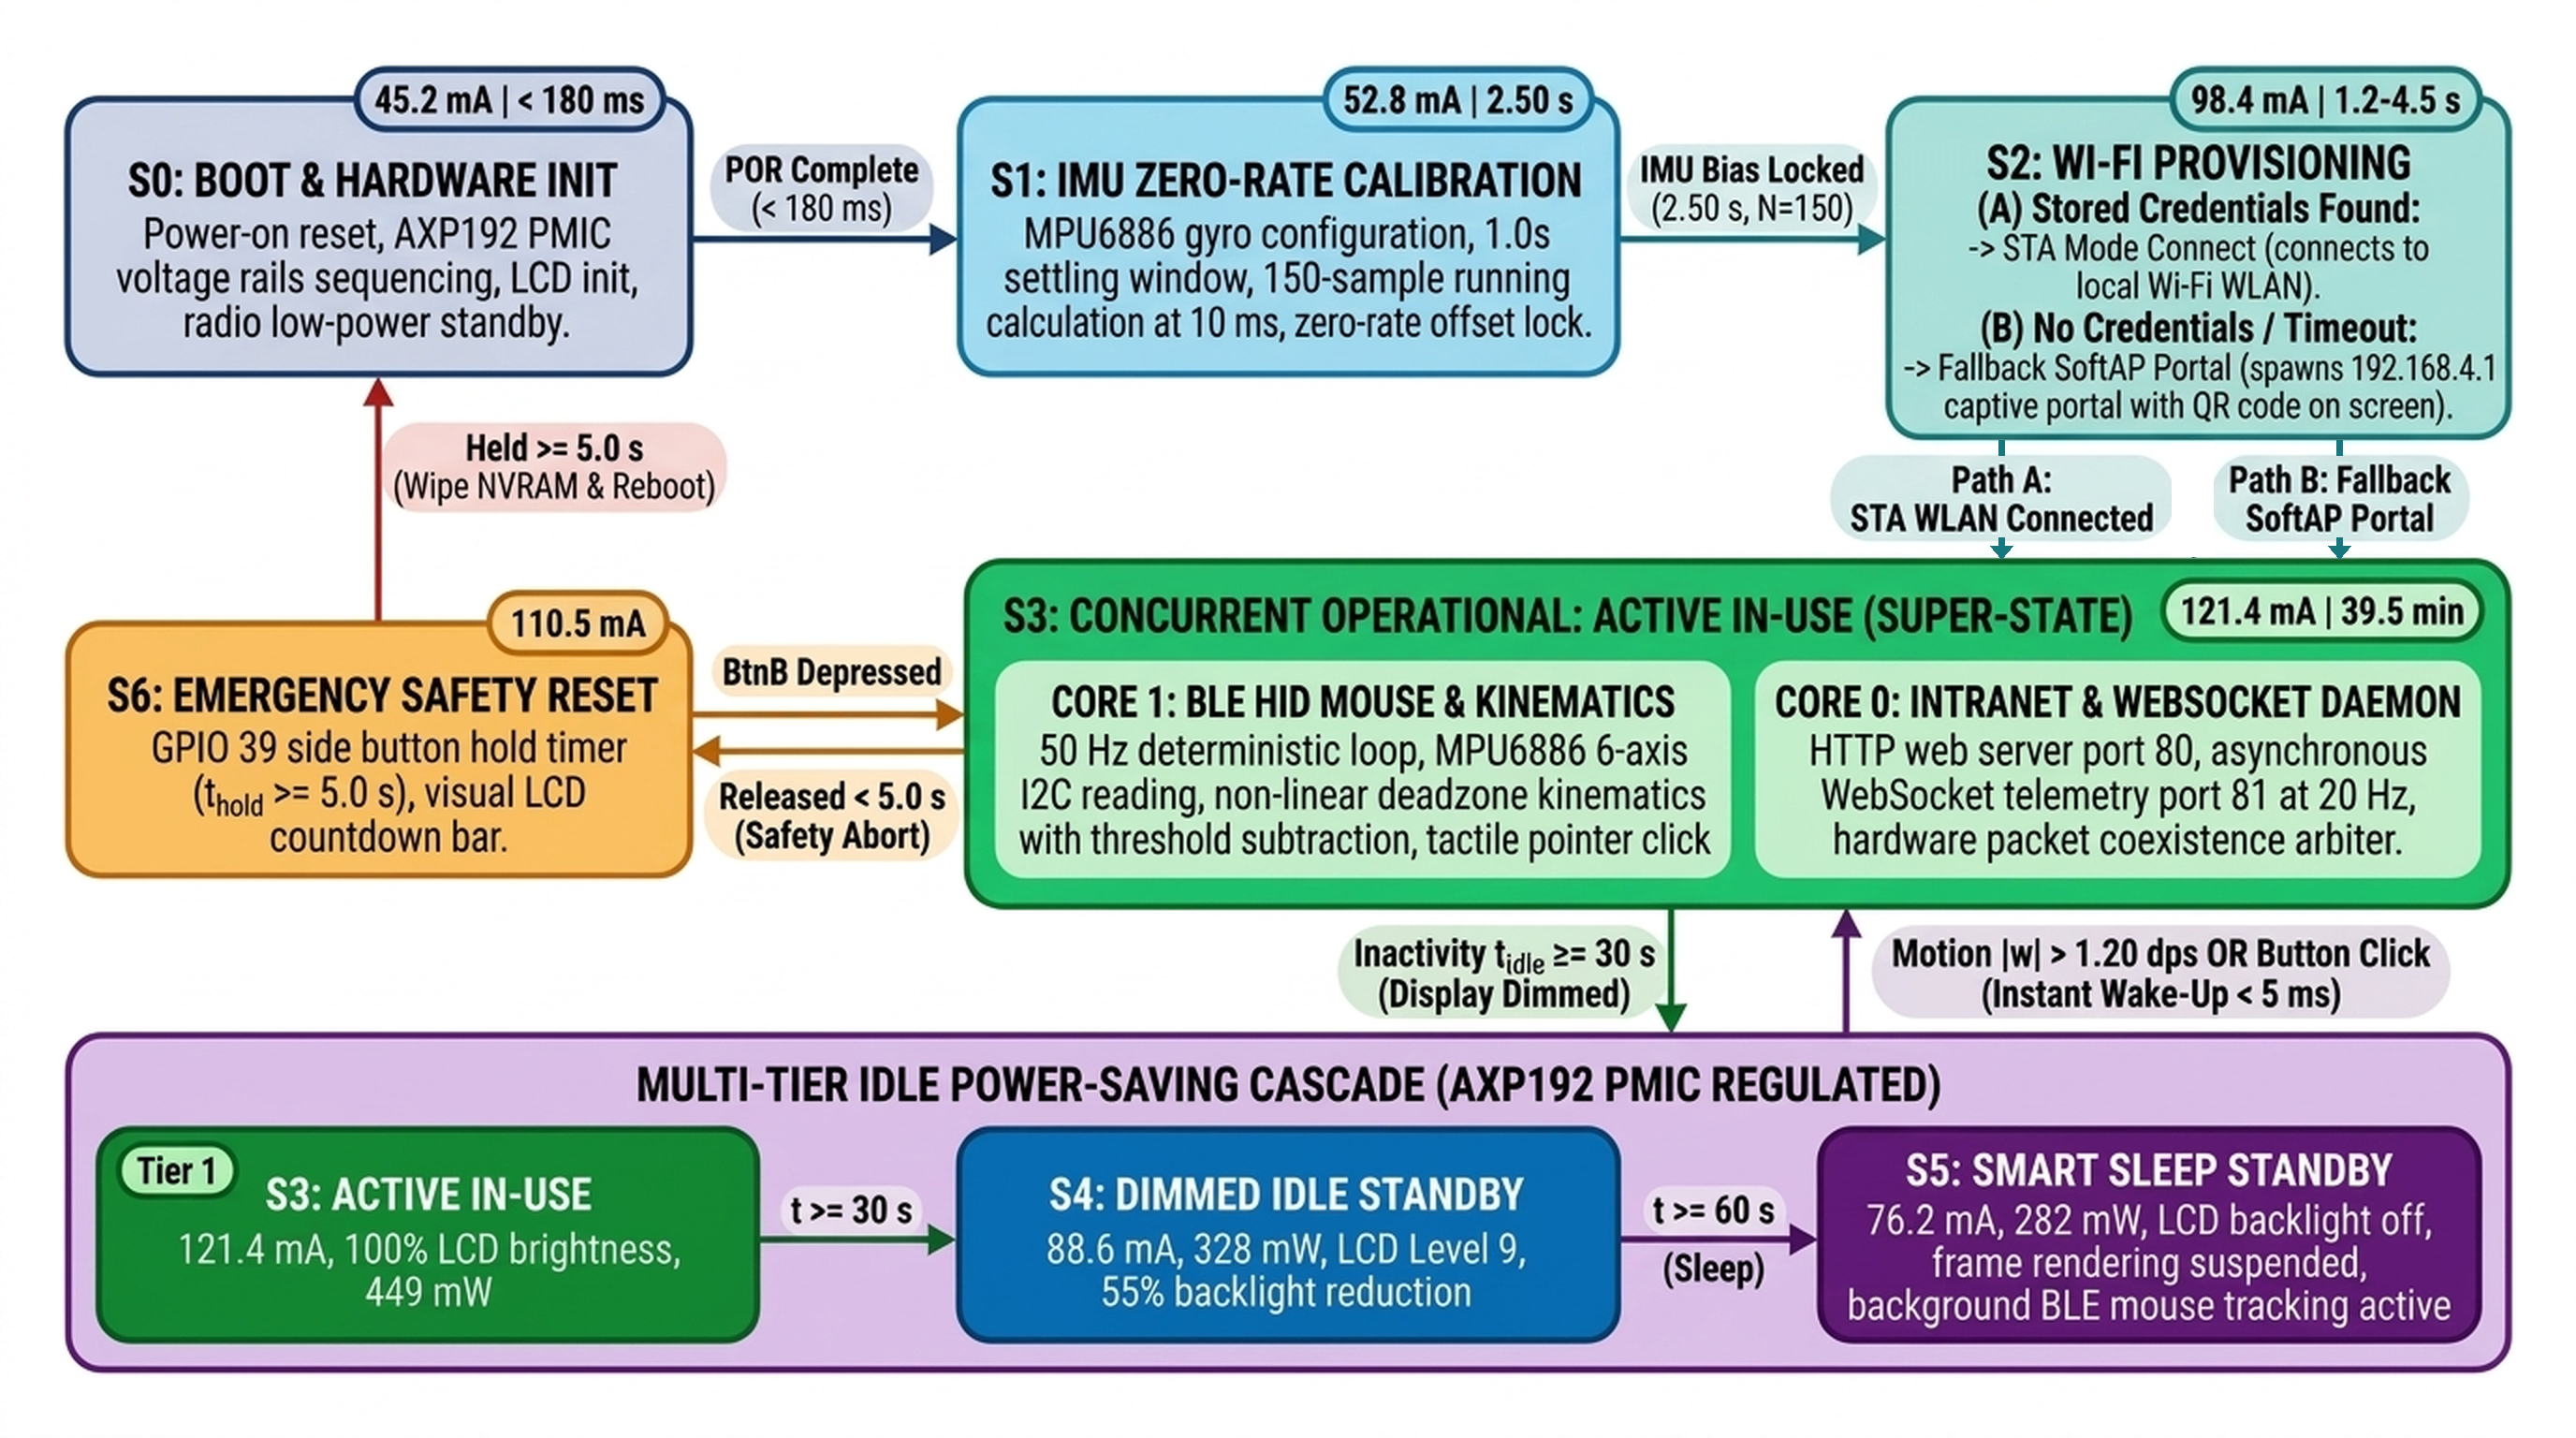
\includegraphics[width=\linewidth]{figures/fig3_firmware_state_machine.png}}{%
\resizebox{\linewidth}{!}{%
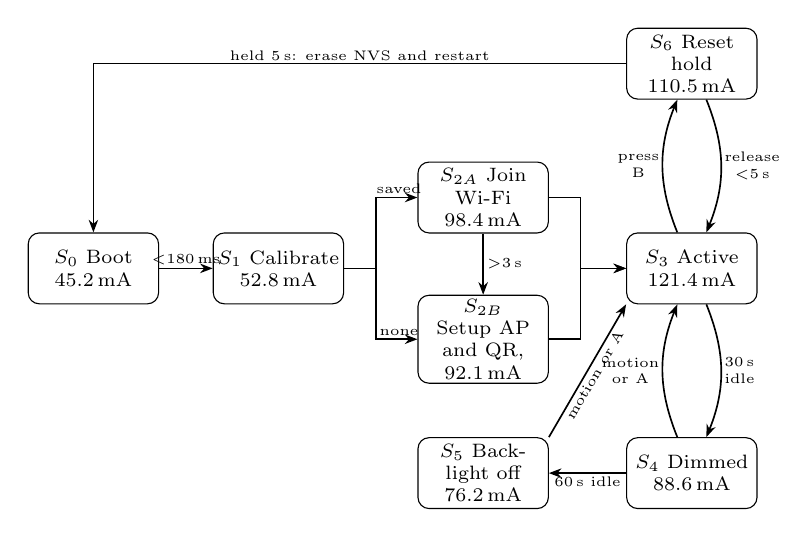
\begin{tikzpicture}[
  font=\scriptsize,
  st/.style={draw, rounded corners=4pt, align=center, minimum height=9mm, text width=15.5mm, inner sep=1.5pt},
  arr/.style={-{Stealth[length=1.6mm]}, semithick},
  lab/.style={font=\tiny, align=center, inner sep=1pt}]
\node[st] (s0)  at (0,0)       {$S_0$ Boot\\45.2\,mA};
\node[st] (s1)  at (2.35,0)    {$S_1$ Calibrate\\52.8\,mA};
\node[st] (s2a) at (4.95,0.9)  {$S_{2A}$ Join Wi-Fi\\98.4\,mA};
\node[st] (s2b) at (4.95,-0.9) {$S_{2B}$ Setup AP\\and QR, 92.1\,mA};
\node[st] (s3)  at (7.6,0)     {$S_3$ Active\\121.4\,mA};
\node[st] (s4)  at (7.6,-2.6)  {$S_4$ Dimmed\\88.6\,mA};
\node[st] (s5)  at (4.95,-2.6) {$S_5$ Backlight off\\76.2\,mA};
\node[st] (s6)  at (7.6,2.6)   {$S_6$ Reset hold\\110.5\,mA};
\draw[arr] (s0) -- node[lab, above] {$<$180\,ms} (s1);
\draw[arr] (s1.east) -- ++(0.4,0) |- node[lab, pos=0.78, above] {saved} (s2a.west);
\draw[arr] (s1.east) -- ++(0.4,0) |- node[lab, pos=0.78, above] {none} (s2b.west);
\draw[arr] (s2a) -- node[lab, right] {$>$3\,s} (s2b);
\draw[arr] (s2a.east) -- ++(0.4,0) |- (s3.west);
\draw[arr] (s2b.east) -- ++(0.4,0) |- (s3.west);
\draw[arr] (s3) to[bend left=22] node[lab, right] {30\,s\\idle} (s4);
\draw[arr] (s4) to[bend left=22] node[lab, left] {motion\\or A} (s3);
\draw[arr] (s4) -- node[lab, below] {60\,s idle} (s5);
\draw[arr] (s5.north east) -- node[lab, sloped, below] {motion or A} (s3.south west);
\draw[arr] (s3) to[bend left=22] node[lab, left] {press\\B} (s6);
\draw[arr] (s6) to[bend left=22] node[lab, right] {release\\$<$5\,s} (s3);
\draw[arr] (s6.west) -| node[lab, pos=0.25, above] {held 5\,s: erase NVS and restart} (s0.north);
\end{tikzpicture}}}
\caption{\IfFileExists{figures/fig3_firmware_state_machine.png}{Firmware state machine and dual-radio concurrency model.}{Firmware state machine with the mean current measured in each state. After calibration, the unit joins a saved network or opens a setup access point; in both cases it then serves the communicator and acts as a BLE mouse. Idle periods dim and then switch off the backlight, and a 5~s hold of Button~B erases the stored settings.}}
\label{fig:fsm}
\end{figure}

% ==== Table II (full width) ===============================================
\begin{table*}[!t]
\caption{Operating States, Active Subsystems, Mean Current, and Transitions}
\label{tab:states}
\centering
\footnotesize
\renewcommand{\arraystretch}{1.15}
\setlength{\tabcolsep}{3.5pt}
\begin{tabular}{@{}l>{\raggedright\arraybackslash}p{6.4cm}r>{\raggedright\arraybackslash}p{4.6cm}l>{\raggedright\arraybackslash}p{1.9cm}@{}}
\toprule
State & Activity and active subsystems & mA & Guard or trigger & Next & Transition time \\
\midrule
$S_0$ & Boot: CPU at 240\,MHz; AXP192 brings up the supply rails; ST7735S display and I\textsuperscript{2}C bus initialized; radios in standby & 45.2 & Power-on reset or software restart & $S_1$ & $<$180\,ms \\
$S_1$ & Bias calibration: MPU-6886 active (41\,Hz filter, $\pm2000$\,\dps); 1.0\,s settling, then 150 samples 10\,ms apart; progress bar on the LCD; radios in standby & 52.8 & Offsets of all three axes stored, Eq.~\eqref{eq:bias} & $S_{2A}$, $S_{2B}$ & 2.50\,s \\
$S_{2A}$ & Join saved network: credentials read from NVS; association and address assignment; HTTP (port 80) and WebSocket (port 81) servers started; BLE advertising & 98.4 & Valid credentials and reachable access point & $S_3$ & 1.20 to 4.50\,s \\
$S_{2B}$ & Setup access point \texttt{CogniLink\_Setup} at 192.168.4.1 with captive portal and QR code on the LCD; servers started; BLE advertising & 92.1 & No credentials, or no association within 3.0\,s & $S_3$ & $<$450\,ms \\
$S_3$ & Active: core~1 runs the 50\,Hz pointing loop (I\textsuperscript{2}C reads, control law, HID reports, Button~A); core~0 runs the HTTP and WebSocket (20\,Hz) servers; LCD level 30 & 121.4 & 30\,s without motion above $\theta$ (to $S_4$); Button~B pressed (to $S_6$) & $S_4$, $S_6$ & $<$2\,ms, $<$1\,ms \\
$S_4$ & Dimmed: both cores active; pointing at 50\,Hz continues; LCD level 9 & 88.6 & 60\,s without motion (to $S_5$); motion above $\theta$ or Button~A (to $S_3$) & $S_5$, $S_3$ & $<$2\,ms, $<$5\,ms \\
$S_5$ & Backlight off: BLE pointing continues; display drawing suspended; motion still monitored & 76.2 & Motion above $\theta$ or Button~A & $S_3$ & $<$5\,ms \\
$S_6$ & Reset hold: Button~B (GPIO39, active low) held; countdown bar on the LCD & 110.5 & Held 5.0\,s: erase NVS and restart (to $S_0$); released earlier: abort (to $S_3$) & $S_0$, $S_3$ & $<$1\,ms \\
\bottomrule
\end{tabular}
\end{table*}

\subsection{Bias Calibration}
\label{sec:calibration}
MEMS gyroscopes have a zero-rate offset that differs between parts and changes with temperature. The MPU-6886 datasheet gives a typical initial tolerance of $\pm1$\,\dps{} and a typical temperature coefficient of $\pm0.01$\,\dps{} per \degC~\cite{mpu6886}. An uncorrected offset of this size would sit close to the deadzone threshold, and without the deadzone it would move the cursor steadily. The firmware therefore estimates the offset at every start-up. After a 1.0~s settling period, it averages $N=150$ readings taken 10~ms apart:
\begin{equation}
\omega_{\mathrm{off},j}=\frac{1}{N}\sum_{i=1}^{N}\omega_{j,i},\qquad j\in\{x,y,z\},
\label{eq:bias}
\end{equation}
where $\omega_{j,i}$ is the $i$th reading on axis $j$ in \dps. During operation, each raw reading is converted to angular rate and corrected:
\begin{align}
\omega_{\mathrm{raw},j}&=\frac{r_j}{S}, \label{eq:raw}\\
\omega_{j}&=\omega_{\mathrm{raw},j}-\omega_{\mathrm{off},j}, \label{eq:corr}
\end{align}
where $r_j\in[-32768,32767]$ is the 16-bit register value and $S=16.4$~LSB per \dps{} is the sensitivity for the $\pm2000$\,\dps{} range. With the noise level estimated in Section~\ref{sec:sensing}, the standard error of the mean of 150 readings is roughly 0.003\,\dps{} when the unit is still, far below the deadzone threshold. The estimate is valid only if the unit does not move during the 2.5~s window, because slow motion during calibration would be absorbed into the offset. The unit should therefore rest on a surface or on a relaxed hand while it starts.

\subsection{Velocity Control Law}
\label{sec:law}
Mapping angular velocity directly to cursor velocity makes the cursor wander whenever residual offset, noise, or small involuntary movement is present. A simple remedy is to zero all rates below a threshold $\theta$ and pass larger rates through unchanged, but this creates a step at the threshold, where a rate just above $\theta$ produces a displacement of $K\theta$ counts per report at once. CogniLink instead subtracts the threshold from the magnitude before applying the gain, so that the output grows from zero. The horizontal and vertical displacements in each report are
\begin{align}
\Delta x&=\operatorname{clip}\!\big(s_x\,\operatorname{sgn}(\omega_z)\max(0,|\omega_z|-\theta)\,K_x\big), \label{eq:dx}\\
\Delta y&=\operatorname{clip}\!\big(s_y\,\operatorname{sgn}(\omega_x)\max(0,|\omega_x|-\theta)\,K_y\big), \label{eq:dy}
\end{align}
with
\begin{equation}
\operatorname{clip}(v)=\max\!\big({-127},\,\min(127,\operatorname{round}(v))\big).
\label{eq:clip}
\end{equation}
Here $\omega_z$ and $\omega_x$ are the corrected rates about the sensor's $z$ and $x$ axes, $\theta=1.20$\,\dps{} is the deadzone threshold, $K_x=K_y=0.60$ counts per \dps{} are the gains, and $s_x,s_y\in\{-1,+1\}$ set the direction of each axis. For the default ring mounting, rotating the finger to the user's right produces a negative $\omega_z$ and must move the cursor right, and raising the finger produces a positive $\omega_x$ and must move the cursor up, toward smaller screen $y$, so $s_x=s_y=-1$ \chk{the specification writes Eq.~(4) with $+\operatorname{sgn}(\omega_z)$ yet describes rightward rotation as giving negative $\omega_z$ and positive $\Delta x$; confirm $s_x$ in the firmware}. Rotation about the sensor's $y$ axis is reported in the telemetry for orientation monitoring but is not used for pointing, which avoids diagonal drift when the user intends to move along one axis. The clip operation keeps each value inside the signed 8-bit range of the report~\cite{usbhid}; without it, a fast movement could overflow the field and reverse the cursor.

Three properties of \eqref{eq:dx} to \eqref{eq:clip} matter in practice. First, because the output is rounded to whole counts, the first nonzero report appears only when $K(|\omega|-\theta)\geq0.5$, that is, at
\begin{equation}
\omega_{\mathrm{on}}=\theta+\frac{1}{2K}\approx2.03\,\text{\dps},
\label{eq:onset}
\end{equation}
so the effective deadzone is wider than $\theta$. Second, above onset the mean cursor speed grows linearly with angular rate,
\begin{equation}
v=f_r\,K\,(|\omega|-\theta),
\label{eq:speed}
\end{equation}
where $f_r=50$~Hz is the report rate, giving 30 counts/s for every \dps{} above $\theta$. For a steady rotation this corresponds to $30(1-\theta/|\omega|)$ counts per degree of rotation, or about 28 counts per degree at 20\,\dps. With a one-to-one mapping of counts to pixels on the host, crossing a 1920-pixel screen at that speed takes about $68^{\circ}$ of rotation; pointer acceleration and other host settings change this mapping. Third, the output saturates at 127 counts when $|\omega|$ reaches $\theta+126.5/K\approx212$\,\dps, which caps the cursor speed at $127f_r=6350$ counts/s. Fig.~\ref{fig:transfer} compares the law with the simple threshold.

The threshold also sets the margin against sensor imperfections. At 1.20\,\dps, $\theta$ is about 39 times the RMS rate noise at the chosen filter setting, and at the typical temperature coefficient a change of more than $100$\,\degC{} would be needed for drift alone to reach $\theta$ after calibration. A side effect of the deadzone is that movement slower than $\omega_{\mathrm{on}}$ never reaches the cursor. A user can therefore bring the finger back to a comfortable position without moving the cursor, much as one lifts and repositions a desk mouse, although at about 2\,\dps{} a $20^{\circ}$ return takes some 10~s. Table~\ref{tab:params} lists the default parameters.

% ==== Figure 5: transfer function (pgfplots, no image file needed) ========
% ALT TEXT: Two plots of counts per report against angular rate. Left, from 0
% to 6 deg/s: the simple threshold jumps to one count at 1.2 deg/s, while
% threshold subtraction starts at 2.03 deg/s and rises in steps that follow
% the unrounded line. Right, from 0 to 250 deg/s: the output rises linearly
% and saturates at 127 counts at about 212 deg/s.
\begin{figure}[!t]
\centering
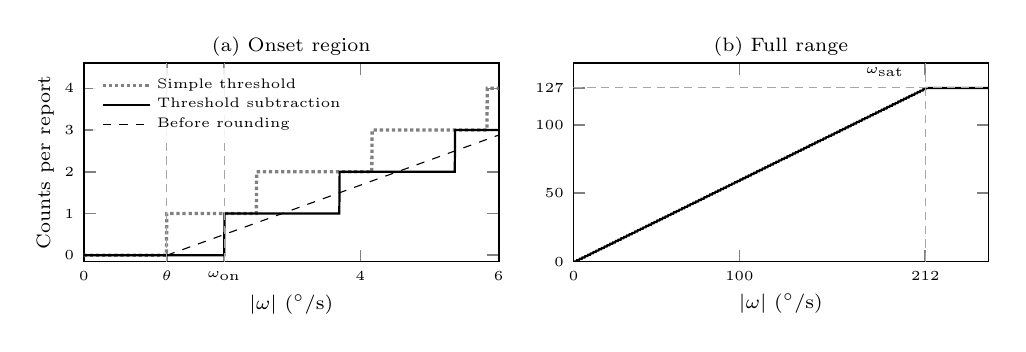
\begin{tikzpicture}
\begin{groupplot}[
  group style={group size=2 by 1, horizontal sep=0.95cm},
  width=0.565\columnwidth, height=4.1cm,
  tick label style={font=\tiny}, label style={font=\scriptsize},
  xlabel style={yshift=2pt}, ylabel style={yshift=-3pt},
  every axis title/.style={font=\scriptsize, at={(0.5,1)}, anchor=south, yshift=-1pt},
  axis line style={semithick}, tick style={semithick}]
\nextgroupplot[title={(a) Onset region}, xmin=0, xmax=6, ymin=-0.15, ymax=4.6,
  xlabel={$|\omega|$ (\dps)}, ylabel={Counts per report},
  xtick={0,1.2,2.03,4,6}, xticklabels={0,$\theta$,$\omega_{\mathrm{on}}$,4,6},
  ytick={0,1,2,3,4},
  legend style={font=\tiny, at={(0.02,0.98)}, anchor=north west, draw=none, fill=white, fill opacity=0.85, text opacity=1, row sep=-2pt},
  legend cell align=left]
\addplot[gray, densely dotted, very thick, samples=1201, domain=0:6] {x<1.2 ? 0 : round(0.6*x)};
\addlegendentry{Simple threshold}
\addplot[black, thick, samples=1201, domain=0:6] {round(0.6*max(0,x-1.2))};
\addlegendentry{Threshold subtraction}
\addplot[black, dashed, thin, samples=2, domain=1.2:6] {0.6*(x-1.2)};
\addlegendentry{Before rounding}
\draw[gray!70, densely dashed, thin] (axis cs:1.2,-0.15) -- (axis cs:1.2,4.6);
\draw[gray!70, densely dashed, thin] (axis cs:2.0333,-0.15) -- (axis cs:2.0333,4.6);
\nextgroupplot[title={(b) Full range}, xmin=0, xmax=250, ymin=0, ymax=145,
  xlabel={$|\omega|$ (\dps)}, xtick={0,100,212,250}, xticklabels={0,100,212,},
  ytick={0,50,100,127}]
\addplot[black, thick, samples=600, domain=0:250] {min(127, round(0.6*max(0,x-1.2)))};
\draw[gray!70, densely dashed, thin] (axis cs:212.03,0) -- (axis cs:212.03,145);
\draw[gray!70, densely dashed, thin] (axis cs:0,127) -- (axis cs:250,127);
\node[font=\tiny, anchor=south east, align=right] at (axis cs:205,128) {$\omega_{\mathrm{sat}}$};
\end{groupplot}
\end{tikzpicture}
\caption{Transfer function of the control law for $\theta=1.20$\,\dps{} and $K=0.60$. (a) Near the threshold, the simple threshold jumps to one count at $\theta$, whereas threshold subtraction starts from zero and gives its first count at $\omega_{\mathrm{on}}\approx2.03$\,\dps{} because of rounding. (b) Over the full range the output grows linearly and saturates at 127 counts at $\omega_{\mathrm{sat}}\approx212$\,\dps. At 50 reports per second, one count per report equals 50 counts/s.}
\label{fig:transfer}
\end{figure}

% ==== Table III ===========================================================
\begin{table}[!t]
\caption{Default Firmware and Communicator Parameters}
\label{tab:params}
\centering
\footnotesize
\setlength{\tabcolsep}{4pt}
\begin{tabular}{@{}>{\raggedright\arraybackslash}p{3.6cm}>{\raggedright\arraybackslash}p{4.4cm}@{}}
\toprule
Parameter & Value \\
\midrule
Gyroscope range, sensitivity & $\pm2000$\,\dps, 16.4~LSB per \dps \\
Digital low-pass filter & \texttt{DLPF\_CFG} = 3 (41~Hz bandwidth) \\
Bias calibration & 1.0\,s settling, $N=150$ samples, 10\,ms apart \\
Deadzone threshold $\theta$ & 1.20\,\dps \\
Gains $K_x$, $K_y$ & 0.60 counts per \dps \\
Axis signs $s_x$, $s_y$ & $-1$, $-1$ (default ring mounting) \\
Report rate $f_r$ & 50~Hz \\
Report range & $-127$ to 127 counts per axis \\
Requested connection interval & 15 to 22.5\,ms, peripheral latency 0 \\
Telemetry & WebSocket on port 81, 20~Hz \\
Display dimming, backlight off & After 30\,s and 60\,s without motion \\
Wi-Fi association timeout & 3.0\,s \\
Reset hold time & 5.0\,s \\
Dwell times & 0.5, 1.0, 2.0, 5.0\,s \\
Dwell ring & $r=13$~px, $C=2\pi r\approx81.68$~px \\
\bottomrule
\end{tabular}
\end{table}

% =========================================================================
\section{Bilingual Communicator}
\label{sec:communicator}
% =========================================================================

\subsection{Delivery as a Self-Hosted Web Page}
The communicator (Fig.~\ref{fig:ui}) is a single-page application written in HTML, CSS, SVG, and JavaScript with no external stylesheets, third-party libraries, or remote hosting. The whole page is stored in the ESP32's flash as a C++ raw string literal (\texttt{const char* INDEX\_HTML}) and served by the unit's HTTP server on port~80, so the communicator travels with the pointer and needs no installation (G2). It offers light and dark themes and a custom assistive cursor. When the unit has joined a local network, any browser on that network can open the page; in setup mode, the host joins the unit's own access point instead. In the second case the host usually has no internet access, so speech then relies on the offline path (Section~\ref{sec:speech}). The page also opens a WebSocket connection to the unit to receive telemetry, including the battery level shown in the interface.

% ==== Figure 6: communicator screenshots (authors' image) =================
% ALT TEXT: Screenshots of the communicator: the English keyboard and the
% Bengali keyboard, each with the message bar, the emergency phrase tray at
% the top, and the dwell ring around a key.
\begin{figure*}[!t]
\centering
\userfig{figures/fig4_communicator_ui.png}{width=\textwidth}{5.6cm}{FIGURE FILE figures/fig4\_communicator\_ui.png\\[2pt] Communicator dashboard across its operating modes, layouts, and themes.}
\caption{The bilingual communicator dashboard across its operating modes, layouts, and themes.}
\label{fig:ui}
\end{figure*}

% ==== Table IV (full width) ================================================
\begin{table*}[!t]
\caption{Physical Target Sizes on Four Displays (mm)}
\label{tab:targets}
\centering
\footnotesize
\setlength{\tabcolsep}{4pt}
\begin{tabular*}{\textwidth}{@{\extracolsep{\fill}}l>{\raggedright\arraybackslash}p{3.3cm}cccc@{}}
\toprule
Element & CSS rule & \shortstack{10.1-inch tablet\\$1920\times1200$, 224 ppi} & \shortstack{15.6-inch laptop\\$1920\times1080$, 141 ppi} & \shortstack{24-inch desktop\\$1920\times1080$, 92 ppi} & \shortstack{43-inch television\\$3840\times2160$, 60\,Hz} \\
\midrule
Character key width & min-width 65\,px; padding 12\,px 20\,px & 9.6 to 10.8 & 13.5 to 15.3 & 20.7 to 23.5 & 37.2 to 42.2 \\
Character key height & min-height 56\,px & 7.1 to 7.6 & 10.1 to 10.8 & 15.5 to 16.6 & 27.8 to 29.8 \\
Space bar & max-width 800\,px; flex-grow 1 & $101.9\times7.6$ & $144.1\times10.8$ & $220.8\times16.6$ & $396.8\times29.8$ \\
Emergency key & Four-column grid, about $280\times65$\,px & $35.7\times8.3$ & $50.4\times11.7$ & $77.3\times18.0$ & $138.9\times32.2$ \\
Layout width & max-width 1200\,px, centered & 152.9 & 216.2 & 331.3 & 595.2 \\
Gap between targets & gap 10\,px & 1.27 & 1.80 & 2.76 & 4.96 \\
\bottomrule
\multicolumn{6}{@{}p{0.98\textwidth}@{}}{\scriptsize Values computed by the authors from the rendered layout. \chk{the tablet column corresponds to about 199 pixels per inch rather than the stated 224, and the television column implies 200\% scaling; state the scaling used for each display and correct the tablet values}}
\end{tabular*}
\end{table*}

% ==== Table V ==============================================================
\begin{table*}[!t]
\caption{Emergency Phrases. The Last Column Gives the Number of Selections Needed to Type Each Sentence Instead (English/Bengali).}
\label{tab:phrases}
\centering
\footnotesize
\renewcommand{\arraystretch}{1.3}
\setlength{\tabcolsep}{3pt}
\begin{tabular*}{\textwidth}{@{\extracolsep{\fill}}cllll>{\raggedright\arraybackslash}p{2.6cm}c@{}}
\toprule
Priority & Label (English) & Spoken (English) & Label (Bengali) & Spoken (Bengali) & Clinical intent & Typed \\
\midrule
1 & I need suction & ``I need suction to clear my throat.'' & \bnimg[0.8]{1} & \bnimg[0.8]{9} & Respiratory and airway clearance & 33/18 \\
2 & I am in pain & ``I am in pain, please help me.'' & \bnimg[0.8]{2} & \bnimg[0.8]{10} & Acute pain & 27/21 \\
3 & I can't breathe & ``I am having trouble breathing.'' & \bnimg[0.8]{3} & \bnimg[0.8]{11} & Dyspnea and ventilator failure & 29/28 \\
4 & Adjust position & ``Please adjust my sitting position.'' & \bnimg[0.8]{4} & \bnimg[0.8]{12} & Posture and pressure ulcer relief & 33/27 \\
5 & I want Water & ``I am thirsty, I need water.'' & \bnimg[0.8]{5} & \bnimg[0.8]{13} & Hydration and nutrition & 25/15 \\
6 & Call Nurse & ``Please call the nurse immediately.'' & \bnimg[0.8]{6} & \bnimg[0.8]{14} & Caregiver and nursing assistance & 33/21 \\
7 & YES & ``Yes.'' & \bnimg[0.8]{7} & \bnimg[0.8]{15} & Affirmation & 3/5 \\
8 & NO & ``No.'' & \bnimg[0.8]{8} & \bnimg[0.8]{16} & Negation & 2/2 \\
\bottomrule
\multicolumn{7}{@{}p{0.98\textwidth}@{}}{\scriptsize Selections were counted as one per key: letters and spaces in English; code points, spaces, and changes to and from the vowel tab in Bengali. Final punctuation and the speak key are excluded.}
\end{tabular*}
\end{table*}

\subsection{Target Sizing}
Larger targets lower the difficulty of each selection~\cite{fitts1954}, and they also give a person with tremor or spasticity more room to hold the pointer still during a dwell. Character keys have a minimum width of 65 CSS pixels, with 12 by 20-pixel padding, and a minimum height of 56 pixels; the space bar grows to at most 800 pixels; emergency keys measure about $280\times65$ pixels in a four-column grid; adjacent targets are separated by 10-pixel gaps; and the layout is centered with a maximum width of 1200 pixels. Table~\ref{tab:targets} gives the resulting physical sizes on four displays. On the 43-inch television, placed 1.5 to 2.5~m from the bed, letter keys are 3.7 to 4.2~cm wide and emergency keys 13.9~cm wide. Because the physical size of a CSS pixel depends on the pixel density of the display and on the scaling set by the host, the layout should be checked on the actual bedside screen.


\subsection{English and Bengali Keyboards}
The English keyboard is a four-row QWERTY layout, with ten digit keys in the first row and ten, nine, and seven letter keys in the next three, together with punctuation; a separate tab provides 32 symbols. Keeping the familiar layout avoids teaching a new one.

The Bengali keyboard follows the traditional order of the alphabet (Fig.~\ref{fig:keyboard}). Its consonant tab, labeled \bnimg[0.95]{21}, has five rows. Each of the first two rows holds two five-letter groups (\textit{varga}) of stops ordered by place of articulation, velar and palatal in Row~1 and retroflex and dental in Row~2. Row~3 holds the labial group followed by five semivowels and sibilants, and Row~4 holds the remaining consonants, the signs anusvara, visarga, and chandrabindu, and the hasanta, so that Rows~1 to 4 carry 39 consonant letters and signs. Row~5 holds the ten dependent vowel signs. A second tab, labeled \bnimg[0.95]{22}, holds the eleven independent vowels and the ten Bengali digits. The aim is that a letter can be found from its group, in the order in which the alphabet is traditionally taught, rather than by visual search.

Conjuncts are typed explicitly. Because each consonant carries an inherent vowel, a cluster cannot be written by placing two consonants side by side; the inherent vowel of the first consonant has to be suppressed with the hasanta, whose key sits in Row~4 among the consonants. The conjunct \textit{k\d{s}a}, for example, is entered as \bnimg[0.95]{17}: the user selects the consonant, the hasanta, and the second consonant, and the browser's text shaping engine, such as HarfBuzz or Core Text, renders the three code points as one conjunct glyph. Other common conjuncts, such as \bnimg[0.95]{19}, are entered the same way. Because every selected key is spoken (Section~\ref{sec:speech}), the hasanta, which has no sound of its own, is announced by name (\bnimg[0.95]{18}). A language key switches between English and Bengali at any time (G3).

% ==== Figure 7: Bengali keyboard schematic (XeLaTeX-rendered PDF) ==========
% Source: figures/bengali_keyboard.tex (compile with XeLaTeX).
% ALT TEXT: Grid of Bengali keys. Rows 1 and 2 hold the velar, palatal,
% retroflex, and dental stops in groups of five. Row 3 holds the labials and
% five semivowels and sibilants. Row 4 holds the remaining consonants, three
% signs, and the highlighted hasanta. Row 5 holds ten vowel signs. A second
% tab holds the eleven vowels and ten digits.
\begin{figure}[!t]
\centering
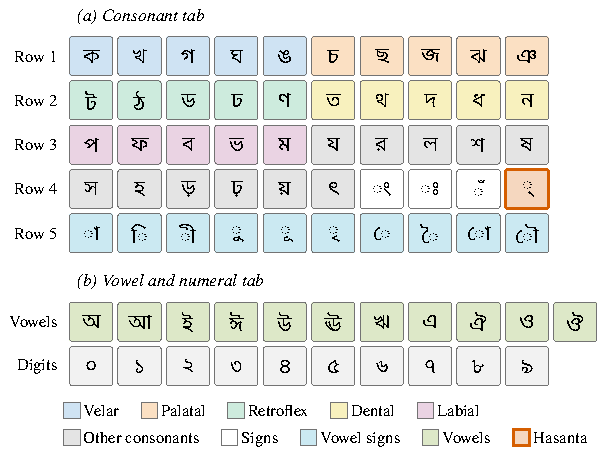
\includegraphics[width=\linewidth]{figures/bengali_keyboard.pdf}
\caption{Key order of the Bengali keyboard. (a) The consonant tab places the stops in groups of five by place of articulation, followed by the semivowels, sibilants, other consonants, signs, and the hasanta (outlined), with the dependent vowel signs in Row~5. (b) The second tab holds the independent vowels and digits. Colors mark the groups; the exact on-screen layout is shown in Fig.~\ref{fig:ui}.}
\label{fig:keyboard}
\end{figure}

\subsection{Dwell Selection}
Every key can be selected by dwelling on it (G1, G6). When the pointer enters a key, the communicator records the time $t_{\mathrm{enter}}$ and starts to fill a ring drawn in Scalable Vector Graphics (SVG) around the key's label. The ring has a radius of $r=13$~px and a circumference $C=2\pi r\approx81.68$~px, and its fill is set through the \texttt{stroke-dashoffset} property,
\begin{equation}
\mathcal{O}(t)=C\left(1-\frac{t-t_{\mathrm{enter}}}{T}\right),
\label{eq:ring}
\end{equation}
where $T$ is the dwell time. The offset is updated on every animation frame through \texttt{requestAnimationFrame}, so the ring fills linearly from empty, $\mathcal{O}=C$, to full, $\mathcal{O}=0$, at which point the key's action fires. If the pointer leaves the key first, a \texttt{mouseleave} event resets the ring and the timer at once, so partial dwells never accumulate. The dwell time can be set to 0.5, 1.0, 2.0, or 5.0~s. The shortest setting matches values that work well in eye typing~\cite{helmert2008,burnham2025}, and the longest guards against accidental selections by users whose pointer often crosses keys while they steer. Users who can press Button~A, or caregivers who assist them, can select without waiting for the dwell.

\subsection{Emergency Phrases}
Eight emergency keys sit at the top of the interface (G4). Each shows a short label in the selected language and speaks a complete sentence when selected (Table~\ref{tab:phrases}). They cover airway clearance, pain, breathing difficulty, positioning, thirst, calling the nurse, and yes and no. Typing the same sentences would take between 2 and 33 selections in English and between 2 and 28 in Bengali. At a dwell time of 1~s, the breathing request alone would need about half a minute of dwell time before any pointer travel, against a single selection from the tray. The phrases were chosen by the authors for an inpatient setting and have not yet been reviewed by clinicians \chk{update this sentence if clinicians reviewed the phrases}.

\subsection{Speech Output}
\label{sec:speech}
Each selected character is spoken as it is entered, and the composed sentence can be spoken in full. After a sentence is spoken, the message box clears after 3~s \chk{the 3~s auto-clear comes from the earlier project brief; confirm that it is still in the current version}. Speech follows two paths. When the host is online, the communicator requests audio for the text from the text-to-speech endpoint of the Google Translate web service over HTTPS and streams it into an HTML5 \texttt{Audio} element. This endpoint is not a documented public interface, offers no service guarantees, and sends every utterance to a third-party server, which matters when utterances describe a patient's health (Section~\ref{sec:privacy}). When the request fails or the host is offline, the communicator falls back to the browser's Web Speech API, which synthesizes speech with voices installed on the host: en-US for English, and bn-BD or bn-IN for Bengali. The API reports through each voice's \texttt{localService} attribute whether synthesis happens on the device or on a remote service~\cite{webspeech}, which allows an application to tell which voices remain usable without a network. Whether an offline Bengali voice exists depends on the host, which Section~\ref{sec:res_compat} examines.

\subsection{Sequential Entry Without Prediction}
\label{sec:noprediction}
The current communicator offers no word prediction. Keys stay where they are, so with practice a user can aim from memory rather than search, and there is no prediction list to read before each selection. Given evidence that reading a prediction list can cost more time than the keystrokes it saves, particularly for users with motor impairment~\cite{koester1994,koester1996}, we chose to establish a stable baseline first and to evaluate Bengali prediction later with metrics suited to the script~\cite{sarcar2015}. The cost of this choice is the number of selections per character, which Section~\ref{sec:disc_bengali} discusses.

% =========================================================================
\section{Evaluation Methodology}
\label{sec:method}
% =========================================================================

\subsection{Units, Hosts, and Conditions}
All measurements were bench tests carried out by the authors, and no participants were involved. Three CogniLink units running the same firmware build \chk{give the firmware version or commit} were tested with the four hosts listed in Table~\ref{tab:hosts}, which cover a desktop workstation, a laptop, a bedside tablet, and a low-cost single-board computer. All displays ran at 60~Hz, so that the frame period was
\begin{equation}
T_{\mathrm{frame}}=\frac{1}{f_{\mathrm{refresh}}}=16.667~\text{ms}.
\label{eq:frame}
\end{equation}
Optical measurements used a Haier 43P7 PRO 43-inch 4K HQLED television with a quantum-dot VA panel ($3840\times2160$ pixels, 60~Hz), connected over HDMI~2.1 and set to Game Mode, which bypasses motion interpolation, dynamic backlight dimming, and edge sharpening \chk{name the host that drove the television}. The room temperature was monitored and held at 28.0\,\degC.

% ==== Table: test hosts =====================================================
\begin{table}[!t]
\caption{Host Platforms Used in the Evaluation}
\label{tab:hosts}
\centering
\footnotesize
\setlength{\tabcolsep}{3pt}
\begin{tabular}{@{}l>{\raggedright\arraybackslash}p{1.45cm}>{\raggedright\arraybackslash}p{3.65cm}>{\raggedright\arraybackslash}p{2.05cm}@{}}
\toprule
Host & Role & Hardware & Software \\
\midrule
A & Desktop workstation & Intel Core i7-12700K (12 cores, 20 threads, up to 5.0\,GHz), 32\,GB DDR4, NVIDIA GeForce RTX 3070 & Windows 11 Pro (64-bit), Chrome 122 \\
B & Laptop & Apple MacBook Pro, M2 Pro (10-core CPU, 16-core GPU), 16\,GB unified memory & macOS Sonoma 14.3, Safari 17.3 \\
C & Bedside tablet & Samsung Galaxy Tab S7, Qualcomm Snapdragon 865+, 6\,GB RAM & Android 13, Chrome 121 \\
D & Low-cost single-board computer & Raspberry Pi 4 Model B, Broadcom BCM2711 (four Cortex-A72 cores, 1.5\,GHz), 4\,GB LPDDR4 & Ubuntu 22.04 LTS, Chromium 120 \\
\bottomrule
\end{tabular}
\end{table}

\subsection{Motion-to-Photon Latency}
\label{sec:method_latency}
Fig.~\ref{fig:testbed} shows the latency testbed. Latency was defined as the time from the moment the firmware detected motion to the moment the screen changed. The firmware configured a spare GPIO pin as a push-pull output and raised it, within 1~$\mu$s, as soon as a corrected angular rate exceeded the deadzone threshold ($|\omega_z|>\theta$ or $|\omega_x|>\theta$). This edge, $t_0$, was recorded on channel~1 of a four-channel, 50~MHz Rigol DS1054Z oscilloscope. A Thorlabs DET36A2 biased silicon PIN photodiode was held against the front of the television, centered over the area where the on-screen cursor was expected to land, under an opaque foam shroud that blocked room light. When the cursor reached that area, the pixels changed from dark to white, and the resulting photocurrent step was recorded on channel~2 as $t_1$. The oscilloscope ran in single-shot mode, edge-triggered on channel~1, and the latency $t_1-t_0$ was read with its timebase cursors. A trained operator rotated the unit by hand about its yaw and pitch axes to start each trial, in place of a mechanical shaker, so that motion onset resembled an intentional gesture. Because $t_0$ is taken after the sensor's own filtering, the measured interval covers the firmware, the BLE link, the host, and the display, but not the sensor and filter delays. A pilot of 50 trials preceded the main series of 10,000 trials \chk{all reported latencies are multiples of 4.17~ms (1/240~s), which matches frame counting in 240~frame/s video rather than oscilloscope timing; confirm the method and explain how 10,000 single-shot trials were acquired}.

% ==== Figure 8: latency testbed (authors' image) ==========================
% ALT TEXT: Photograph or diagram of the latency testbed: the wearable unit
% with a GPIO marker wired to the oscilloscope, the photodiode on the
% television screen under a shroud, and the host computer.
\begin{figure}[!t]
\centering
\userfig{figures/fig5_testbed_setup.png}{width=\linewidth}{5.0cm}{FIGURE FILE figures/fig5\_testbed\_setup.png\\[2pt] Latency testbed: GPIO marker from the unit to oscilloscope channel 1; photodiode on the television screen to channel 2; host driving the television over HDMI.}
\caption{Optoelectronic latency testbed and signal path. A GPIO marker raised by the firmware when motion is detected ($t_0$) and the output of a photodiode on the television screen ($t_1$) are recorded on two oscilloscope channels.}
\label{fig:testbed}
\end{figure}

\subsection{Resting Stability}
Cursor stability at rest was recorded in ten runs of 60~s. In Runs~1 to 5 the deadzone was disabled ($\theta=0$), and in Runs~6 to 10 it was set to its default of 1.20\,\dps. During each run the unit was held stationary \chk{state whether it lay on the bench or was worn on a resting hand}, and the host logged the cursor position $(X(t),Y(t))$ at 50~Hz on a $1920\times1080$-pixel canvas, giving 3000 samples per run \chk{a headless browser does not receive pointer events from a physical mouse; describe the logging tool}. Drift was quantified as the Euclidean displacement from the starting position,
\begin{equation}
D(t)=\sqrt{\big[X(t)-X(0)\big]^2+\big[Y(t)-Y(0)\big]^2},
\label{eq:drift}
\end{equation}
and as the mean drift speed over a run of duration $\Delta t$,
\begin{equation}
v_{\mathrm{drift}}=\frac{D(t_{\mathrm{end}})}{\Delta t}.
\label{eq:vdrift}
\end{equation}

\subsection{HID Report Timing}
The intervals between successive HID reports were recorded for 10,000 consecutive reports with an Ellisys Bluetooth Explorer 400 over-the-air sniffer, supplemented by host-side input timestamps (\texttt{evhz} on Linux and \texttt{GetRawInputBuffer} on Windows) \chk{state which source the reported intervals come from}.

\subsection{Dwell Timing}
Dwell accuracy was measured over 10,000 dwell selections, 2,500 at each dwell time. For each selection the communicator recorded, with \texttt{performance.now()}, the time at which the pointer entered the key and the time at which the selection fired, and the timing error was the difference between the measured and the nominal dwell time \chk{state how pointer entries were produced, by the device or by scripted events}.

\subsection{Power}
Current was measured with a Keysight 34465A 6.5-digit digital multimeter in series with the 3.7~V cell, sampling at 100~Hz, in each operating state and in two further configurations: BLE pointing with Wi-Fi disabled, and deep standby with both radios off. Battery runtime was estimated from the mean current $I$ as
\begin{equation}
T_{\mathrm{run}}=\frac{\eta\,C}{I},
\label{eq:runtime}
\end{equation}
with a nominal capacity $C=80$~mAh and a usable fraction $\eta=0.95$ down to the 3.30~V cutoff \chk{if discharge runtimes from 4.20 to 3.30~V were measured, report them here; the runtimes in the specification equal $C/I$ exactly, which suggests they were calculated}.

\subsection{Speech Onset}
Speech onset latency, from the selection event to the start of sound, was measured over 10,000 utterances, 2,500 for each combination of engine (cloud or offline) and language, with a studio condenser microphone connected to an audio analyzer \chk{give the network type and speed for the cloud tests}.

\subsection{Compatibility}
On each host we checked BLE pairing without a driver, continuous pointing, Button~A clicks, dwell selection, rendering of typed Bengali conjuncts, offline Bengali speech, and whether the pointer could operate two third-party web communicators, Cboard~\cite{cboard} and AsTeRICS Grid~\cite{astericsgrid}.

\subsection{Data Analysis and Availability}
Results are reported as mean $\pm$ standard deviation (SD), with the median, interquartile range (IQR), range, and a normal-approximation 95\% confidence interval (CI) of the mean where available. The drift comparison used a one-sample $t$-test of the deadzone-off displacements against zero. Because every deadzone-on displacement was exactly zero, this test is identical to Welch's test between the two conditions. The raw data files (\path{latency_10000_trials.csv}, \path{hid_report_10000_packets.csv}, \path{dwell_10000_trials.csv}, and \path{speech_onset_10000_trials.csv}), together with the firmware, communicator, and cradle files, will be released at \tbd{repository URL} under \tbd{license}.

% =========================================================================
\section{Results}
\label{sec:results}
% =========================================================================

Table~\ref{tab:timing} summarizes the timing measurements, and Fig.~\ref{fig:bench} shows their distributions.

% ==== Table VI =============================================================
\begin{table*}[!t]
\caption{Timing Measurements (ms). CI: 95\% Confidence Interval of the Mean; n/r: Not Reported.}
\label{tab:timing}
\centering
\footnotesize
\begin{tabular}{@{}llrrrrrrc@{}}
\toprule
Measure & Condition & $n$ & Mean & SD & Median & Min & Max & 95\% CI \\
\midrule
Motion-to-photon latency & Host to 60\,Hz television & 10,000 & 44.35 & 4.36 & 45.83 & 33.33 & 54.17 & [44.26, 44.43] \\
 & Pilot & 50 & 44.83 & 4.64 & 45.83 & 33.33 & 54.17 & [43.54, 46.12] \\
HID report interval & BLE link & 10,000 & 20.54 & 1.43 & n/r & 16.50 & 25.42 & [20.51, 20.57] \\
\addlinespace
Dwell timing error & 0.5\,s dwell & 2,500 & $+$1.42 & 3.27 & n/r & $-$6.00 & $+$13.76 & [1.29, 1.55] \\
 & 1.0\,s dwell & 2,500 & $+$1.90 & 3.61 & n/r & $-$6.00 & $+$14.00 & [1.76, 2.04] \\
 & 2.0\,s dwell & 2,500 & $+$2.26 & 3.93 & n/r & $-$6.00 & $+$14.00 & [2.10, 2.41] \\
 & 5.0\,s dwell & 2,500 & $+$4.04 & 4.99 & n/r & $-$6.00 & $+$14.00 & [3.84, 4.24] \\
 & All dwell times & 10,000 & $+$2.41 & 4.13 & n/r & $-$6.00 & $+$14.00 & [2.32, 2.49] \\
\addlinespace
Speech onset & Cloud, English & 2,500 & 319.05 & 24.38 & 318.52 & 244.59 & 392.25 & [318.09, 320.00] \\
 & Cloud, Bengali & 2,500 & 354.37 & 28.56 & 354.10 & 269.19 & 439.11 & [353.25, 355.49] \\
 & Offline, English & 2,500 & 43.62 & 4.88 & 43.48 & 29.19 & 58.05 & [43.42, 43.81] \\
 & Offline, Bengali & 2,500 & 58.27 & 6.30 & 58.09 & 39.82 & 76.66 & [58.02, 58.52] \\
\bottomrule
\end{tabular}
\end{table*}

% ==== Figure 9: benchmark results (authors' image) ========================
% Check that the panel order (a) to (f) below matches your figure file.
% ALT TEXT: Six panels: latency histogram; cursor displacement over 60 s with
% the deadzone off and on; dwell timing error at four dwell times; speech
% onset for four engine and language combinations; distribution of intervals
% between HID reports; current and runtime in each operating scenario.
\begin{figure*}[!t]
\centering
\userfig{figures/fig6_benchmarks.png}{width=\textwidth}{8.0cm}{FIGURE FILE figures/fig6\_benchmarks.png\\[2pt] Benchmark panels (a) to (f) as described in the caption.}
\caption{Benchmark results. (a) Distribution of motion-to-photon latency, with the mean marked, the 95\% confidence band shaded, and an inset box plot. (b) \chk{describe panel (b); the specification does not refer to it}. (c) Dwell timing accuracy at the four dwell times. (d) Speech onset latency for cloud and offline engines in English and Bengali. (e) Intervals between successive HID reports with a fitted Gaussian. (f) Battery discharge from 4.20 to 3.30~V.}
\label{fig:bench}
\end{figure*}

\subsection{Motion-to-Photon Latency}
Over 10,000 trials, motion-to-photon latency was $44.35\pm4.36$~ms (95\% CI 44.26 to 44.43~ms), with a median of 45.83~ms, an IQR of 4.17~ms, and a range of 33.33 to 54.17~ms (Fig.~\ref{fig:bench}(a)). The 50-trial pilot gave $44.83\pm4.64$~ms, consistent with the main series.

To see where this time goes, we model the latency as the sum of the delays that follow $t_0$:
\begin{equation}
L=t_{\mathrm{fw}}+t_{\mathrm{BLE}}+t_{\mathrm{host}}+t_{\mathrm{wait}}+t_{\mathrm{scan}}+t_{\mathrm{disp}},
\label{eq:latency}
\end{equation}
where $t_{\mathrm{fw}}$ is the firmware time from detection to queueing the report, $t_{\mathrm{BLE}}$ the wait for the next connection event plus the time on air, $t_{\mathrm{host}}$ the processing in the host's Bluetooth stack, HID driver, and pointer pipeline, $t_{\mathrm{wait}}$ the wait for the next display refresh, $t_{\mathrm{scan}}$ the time for the scan-out to reach the photodiode, and $t_{\mathrm{disp}}$ the television's own processing and the response of its pixels. For a photodiode at row $y$ of a display with $Y$ rows,
\begin{equation}
t_{\mathrm{scan}}(y)=\frac{y}{Y}\,T_{\mathrm{frame}},
\label{eq:scan}
\end{equation}
which is 8.33~ms at mid-screen ($y=1080$ of $Y=2160$).

Table~\ref{tab:budget} lists the terms. Sensing happens before $t_0$ and is therefore outside the measured interval. It comprises the delay of the gyroscope's filter and the I\textsuperscript{2}C burst read of the six gyroscope registers (0x43 to 0x48)~\cite{mpu6886}, which takes 81 clock cycles, or about 0.2~ms, at 400~kHz. The firmware time from detection to queueing the report, measured with the ESP-IDF microsecond timer (\texttt{esp\_timer\_get\_time()}), was 0.2 to 0.5~ms; it covers unit conversion, bias correction, the deadzone, gain, clipping, and the hand-over to the NimBLE queue. Event Tracing for Windows and Chromium tracing on Host~A gave 2.5 to 5.5~ms for the host path: 0.6 to 1.2~ms for parsing the Bluetooth packet, 0.4 to 0.8~ms for dispatching the pointer event, 0.8 to 1.5~ms for the browser's event handling and compositing, and 0.7 to 2.0~ms for the swap-chain present call. The two waits are set by clocks that run independently of the motion. A report waits on average half a connection interval, 7.5 to 11.25~ms for intervals of 15 to 22.5~ms, plus less than 0.4~ms on air, and a cursor update waits on average half a frame, 8.33~ms, for the next refresh. Together with the scan-out, these terms account for a mean of 28.8 to 32.5~ms. The remaining 11.8 to 15.6~ms of the measured mean is attributed to the television. It includes the gray-to-gray transition of the VA panel, 6.5 to 8.5~ms according to the photodiode rise, and the processing in Game Mode, which we did not measure separately \chk{the measured spread is narrower than this model allows: the refresh wait alone, uniform over one frame, has an SD of 4.81~ms, above the measured SD of 4.36~ms, and the BLE wait adds further spread; report the negotiated connection interval and recheck the latency data}.

% ==== Table VII ===========================================================
\begin{table}[!t]
\caption{Latency Budget From Detected Motion to Light at Mid-Screen}
\label{tab:budget}
\centering
\footnotesize
\setlength{\tabcolsep}{3pt}
\begin{tabular}{@{}>{\raggedright\arraybackslash}p{2.0cm}>{\raggedright\arraybackslash}p{3.15cm}cc@{}}
\toprule
Stage & Basis & Range (ms) & Mean (ms) \\
\midrule
Firmware, $t_{\mathrm{fw}}$ & Measured, ESP-IDF timer & 0.2 to 0.5 & 0.3 \\
BLE link, $t_{\mathrm{BLE}}$ & Model: uniform wait over one 15 to 22.5\,ms interval, plus air time & 0.2 to 22.9 & 7.8 to 11.6 \\
Host path, $t_{\mathrm{host}}$ & Measured, Event Tracing for Windows and Chromium tracing on Host~A & 2.5 to 5.5 & 4.0 \\
Refresh wait, $t_{\mathrm{wait}}$ & Model: uniform over one frame & 0 to 16.7 & 8.3 \\
Scan-out, $t_{\mathrm{scan}}$ & Model: \eqref{eq:scan} at mid-screen & 8.3 & 8.3 \\
\midrule
Modeled subtotal & & 11.2 to 53.9 & 28.8 to 32.5 \\
Television, $t_{\mathrm{disp}}$ & Inferred: measured mean minus subtotal; includes a 6.5 to 8.5\,ms panel transition & n/m & 11.8 to 15.6 \\
\midrule
Measured total & Photodiode, 10,000 trials & 33.3 to 54.2 & 44.35 \\
\bottomrule
\multicolumn{4}{@{}l@{}}{\scriptsize n/m: not measured.}
\end{tabular}
\end{table}

\subsection{Resting Stability}
Table~\ref{tab:drift} lists the ten runs. With the deadzone disabled, the cursor moved $25.44\pm4.16$~px over 60~s (range 21.36 to 30.66~px), a mean drift speed of $0.424\pm0.069$~px/s, with no consistent direction across runs. With the deadzone enabled, the cursor did not move in any of the 15,000 samples, and the displacement was 0.00~px in all five runs. The difference between the conditions was significant ($t(4)=13.69$, $p=1.7\times10^{-4}$), although with zero variance in one condition the test adds little to the observation that the deadzone removed all measurable drift at rest \chk{the summary row of the specification (25.14 $\pm$ 3.64~px; $t=15.45$; $p=7.82\times10^{-5}$) does not match its own per-run values; the figures given here are recomputed from the per-run values}.

% ==== Table VIII ===========================================================
\begin{table}[!t]
\caption{Cursor Displacement After 60 s at Rest (28.0\,\degC, 3000 Samples per Run)}
\label{tab:drift}
\centering
\footnotesize
\setlength{\tabcolsep}{3pt}
\begin{tabular}{@{}lcrrrr@{}}
\toprule
Run & $\theta$ (\dps) & $\Delta X$ (px) & $\Delta Y$ (px) & $D$ (px) & $v_{\mathrm{drift}}$ (px/s) \\
\midrule
1 & 0 & $+$18.40 & $-$12.10 & 22.02 & 0.367 \\
2 & 0 & $-$24.20 & $+$15.80 & 28.90 & 0.482 \\
3 & 0 & $+$11.60 & $+$21.30 & 24.25 & 0.404 \\
4 & 0 & $-$19.70 & $-$23.50 & 30.66 & 0.511 \\
5 & 0 & $+$15.30 & $-$14.90 & 21.36 & 0.356 \\
6 to 10, each & 1.20 & 0.00 & 0.00 & 0.00 & 0.000 \\
\midrule
\multicolumn{4}{@{}l}{Runs 1 to 5, mean $\pm$ SD} & $25.44\pm4.16$ & $0.424\pm0.069$ \\
\multicolumn{4}{@{}l}{Runs 6 to 10, mean $\pm$ SD} & $0.00\pm0.00$ & $0.000\pm0.000$ \\
\bottomrule
\end{tabular}
\end{table}

\subsection{Report Timing}
Over 10,000 consecutive reports, the interval between reports was $20.54\pm1.43$~ms (95\% CI 20.51 to 20.57~ms), an effective rate of 48.7~Hz against the nominal 50~Hz, with a range of 16.50 to 25.42~ms, equivalent to 60.6 to 39.3~Hz (Fig.~\ref{fig:bench}(e)). No reports were lost \chk{over the air, notifications can leave only at connection events, so sniffer intervals should cluster at multiples of the connection interval rather than spread continuously around 20.5~ms; state the negotiated interval, the source of these timestamps, and how lost reports were detected}.

\subsection{Dwell Timing}
Dwell selections fired $2.41\pm4.13$~ms later than nominal over all 10,000 selections, with the mean error rising from 1.42~ms at 0.5~s to 4.04~ms at 5.0~s (Table~\ref{tab:timing}; Fig.~\ref{fig:bench}(c)). Relative to the nominal dwell, the mean error was 0.28\% at 0.5~s, 0.19\% at 1.0~s, 0.11\% at 2.0~s, and 0.08\% at 5.0~s, or 0.17\% on average. Individual errors ranged from $-6.00$ to $+14.00$~ms \chk{a negative error means that a selection fired before the dwell had elapsed, and the same minimum ($-6.00$~ms) and maximum (about $+14.00$~ms) appear at every dwell time; if the dwell is checked once per 60~Hz frame, errors between 0 and 16.7~ms with a mean near 8~ms would be expected; confirm how both timestamps were taken}.

\subsection{Power and Runtime}
Table~\ref{tab:power} lists the measured currents and the runtimes estimated with \eqref{eq:runtime}. With Wi-Fi, BLE, and the display at full brightness, the unit drew 121.4~mA (449~mW at 3.7~V), which gives an estimated 38~min of operation from the 80~mAh cell. Dimming and then switching off the backlight lowered the current to 88.6 and 76.2~mA and extended the estimate to 52 and 60~min. Disabling Wi-Fi had the largest effect. As a BLE-only mouse with the display off, the unit drew 41.5~mA, for an estimated 110~min, and in deep standby it drew 2.1~mA, for about 36~h. Wi-Fi with its servers therefore accounts for about 35~mA of the 76.2~mA drawn in $S_5$. For longer sessions the unit can run from USB power. A 500~mAh external battery would add roughly 4~h at the active-state current, before conversion losses.

% ==== Table IX (full width) ================================================
\begin{table*}[!t]
\caption{Measured Current and Estimated Runtime From an 80~mAh Cell}
\label{tab:power}
\centering
\footnotesize
\setlength{\tabcolsep}{4pt}
\begin{tabular*}{\textwidth}{@{\extracolsep{\fill}}lccccrr>{\raggedright\arraybackslash}p{3.9cm}@{}}
\toprule
Scenario & Wi-Fi & BLE & Display & $I$ (mA) & $P$ (mW) & $T_{\mathrm{run}}$ & Intended use \\
\midrule
Active ($S_3$) & Connected & Connected & Level 30 & 121.4 & 449.2 & 37.6\,min & Continuous conversation at the bedside \\
Dimmed ($S_4$) & Connected & Connected & Level 9 & 88.6 & 327.8 & 51.5\,min & Waiting between phrases \\
Backlight off ($S_5$) & Connected & Connected & Off & 76.2 & 281.9 & 59.8\,min & Resting, with pointing ready \\
BLE only & Disabled & Connected & Off & 41.5 & 153.6 & 109.9\,min & Pointer for third-party AAC \\
Deep standby & Disabled & Disabled & Controller sleep & 2.1 & 7.8 & 36.2\,h & Long standby at the bedside \\
\bottomrule
\multicolumn{8}{@{}p{0.98\textwidth}@{}}{\scriptsize Wi-Fi connected: HTTP and WebSocket servers running. BLE connected: HID link active. Power at the nominal 3.7~V. Runtime from \eqref{eq:runtime} with $C=80$~mAh and $\eta=0.95$; without the 0.95 factor the values are 39.5, 54.2, 63.0, and 115.7~min and 38.1~h.}
\end{tabular*}
\end{table*}

\subsection{Speech Onset}
Offline synthesis started much sooner than cloud synthesis (Table~\ref{tab:timing}; Fig.~\ref{fig:bench}(d)). The cloud path took $319.05\pm24.38$~ms in English and $354.37\pm28.56$~ms in Bengali, whereas the offline path took $43.62\pm4.88$~ms and $58.27\pm6.30$~ms, reductions of 86.3\% and 83.6\%. With both engines, Bengali took longer than English, by 35~ms in the cloud and 15~ms offline.

\subsection{Compatibility}
\label{sec:res_compat}
All checks passed on all four hosts (Table~\ref{tab:compat}). The unit paired as a BLE mouse with Windows, macOS, Android, and Linux (through the BlueZ stack) without drivers. Pointing, Button~A clicks, and dwell selection worked on each host, and all four browsers rendered typed conjuncts correctly. Each host offered an offline Bengali voice \chk{list the voice name on each host and its \texttt{localService} value, and confirm that the offline tests were run with the network disconnected}. The pointer also operated Cboard and AsTeRICS Grid on every host \chk{state whether selections in Cboard used Button~A, dwell, or another method}.

% ==== Table X ==============================================================
\begin{table}[!t]
\caption{Compatibility Across Host Platforms}
\label{tab:compat}
\centering
\footnotesize
\setlength{\tabcolsep}{3pt}
\begin{tabular*}{\columnwidth}{@{\extracolsep{\fill}}>{\raggedright\arraybackslash}p{2.6cm}cccc@{}}
\toprule
Check & Host A & Host B & Host C & Host D \\
\midrule
BLE pairing, no driver & Pass & Pass & Pass & Pass \\
Continuous pointing & Pass & Pass & Pass & Pass \\
Button A click & Pass & Pass & Pass & Pass \\
Dwell selection & Pass & Pass & Pass & Pass \\
Bengali conjunct rendering & Pass & Pass & Pass & Pass \\
Offline Bengali voice & bn-BD, bn-IN & bn-IN & Google TTS & eSpeak NG \\
Cboard & Pass & Pass & Pass & Pass \\
AsTeRICS Grid & Pass & Pass & Pass & Pass \\
\bottomrule
\multicolumn{5}{@{}p{0.97\columnwidth}@{}}{\scriptsize A: Windows 11, Chrome 122. B: macOS 14.3, Safari 17.3. C: Android 13, Chrome 121. D: Ubuntu 22.04 on Raspberry Pi 4, Chromium 120.}
\end{tabular*}
\end{table}

\subsection{Cost}
Table~\ref{tab:bom} itemizes the hardware, which costs US\$15.00 (1,770~BDT) at single-unit prices in Bangladesh \chk{give the suppliers and the date of the prices}, excluding the host device. This is 97.5\% below the price of the GlassOuse head mouse (US\$599)~\cite{glassouse}, 98.5\% below the estimated cost of the Quha Zono (US\$999)~\cite{montechquha}, and 98.8\% below that of the PCEye~5 eye tracker (US\$1,249)~\cite{montechpceye}. These comparisons cover the hardware price only. They do not account for support, warranty, durability, or the software bundled with commercial devices.

% ==== Table XI ============================================================
\begin{table}[!t]
\caption{Bill of Materials (Single-Unit Prices)}
\label{tab:bom}
\centering
\footnotesize
\setlength{\tabcolsep}{3pt}
\begin{tabular}{@{}>{\raggedright\arraybackslash}p{2.0cm}>{\raggedright\arraybackslash}p{1.75cm}>{\raggedright\arraybackslash}p{2.35cm}rr@{}}
\toprule
Item & Source & Role & USD & BDT \\
\midrule
M5StickC module & M5Stack development kit & Controller, IMU, power management, display, battery & 12.50 & 1,475 \\
Silicone strap, hook-and-loop fastener & Generic supplier & Holds the unit on the body; washable & 0.85 & 100 \\
PETG cradle & In-house FDM printing & Mount for all five sites & 0.45 & 53 \\
USB-A to USB-C cable, 1~m & Generic retail & Programming, charging, and power & 1.20 & 142 \\
\midrule
Total & & & 15.00 & 1,770 \\
\bottomrule
\end{tabular}
\end{table}

% =========================================================================
\section{Discussion}
\label{sec:discussion}
% =========================================================================

\subsection{Latency in Context}
MacKenzie and Ware found that lag measurably slowed pointing at 75~ms and slowed it severely at 225~ms~\cite{mackenzie1993}. The mean latency measured here, about 44~ms from detected motion to light on the screen, lies between their 25~ms and 75~ms conditions. The delay from the physical start of motion is a few milliseconds longer, because the sensor's filter acts before $t_0$. Since a dwell selection with CogniLink takes 0.5 to 5~s, latency is unlikely to be the main limit on communication speed, although its effect on closed-loop steering by users with motor impairment remains to be measured.

The latency budget (Table~\ref{tab:budget}) shows where improvement is possible. The BLE wait and the display account for most of the delay, whereas the firmware contributes less than 1~ms. Requesting the shortest standard connection interval of 7.5~ms~\cite{btcore62} would cut the mean BLE wait to about 3.75~ms and save 4 to 8~ms, at the cost of more radio activity and current, and a 120~Hz display would halve both the refresh wait and the scan-out time. Bluetooth Core~6.2 adds connection intervals well below 7.5~ms~\cite{btcore62}, but the Bluetooth~4.2 radio of the ESP32-PICO-D4~\cite{esp32picod4} cannot use them.

\subsection{Deadzone Design}
The deadzone did what it was designed to do: with it, the cursor did not move at rest, and without it, the cursor drifted by about 25~px per minute. Two observations qualify this result. First, the drift measured with $\theta=0$ cannot come from sensor noise alone. Because \eqref{eq:clip} rounds every report, a rate must exceed $1/(2K)\approx0.83$\,\dps{} to produce even one count, about 27 times the RMS noise. The observed drift therefore reflects either small real movements of the unit or a firmware path that carries sub-count remainders from one report to the next \chk{state which; if remainders are carried over, add this step to Eqs.~(4) to (6)}. Second, the deadzone that removes drift also hides slow intentional movement, since nothing reaches the cursor below about 2\,\dps{} \eqref{eq:onset}. This trade-off matters for people whose movements are slow and small, as in advanced ALS. A per-user threshold, set from the variability measured while the user rests, together with a per-user gain, would let the same law serve both stable and weak users, and both could be set from the communicator, which already exchanges data with the unit over WebSocket.

The deadzone is not a tremor filter. Involuntary movements faster than $\theta$, such as tremor or spasms, pass through \eqref{eq:dx} and \eqref{eq:dy} and are limited only by saturation, which prevents wrap-around but not unwanted motion. Dwell selection partly compensates, because a key is selected only if the pointer stays on it for the full dwell, but users with marked tremor may need additional filtering, such as a low-pass stage with a cut-off below the tremor band, at the cost of added latency.

\subsection{Dwell Timing and Choice of Dwell Time}
The measured dwell errors were a few milliseconds, below 0.3\% of the nominal dwell, so timing accuracy does not limit dwell selection. The open question is which dwell times suit body-worn pointing. Eye-typing studies favor about 500~ms~\cite{helmert2008} and show that users shorten the dwell with practice~\cite{majaranta2009}, and a meta-analysis reports 500 to 600~ms as a common balance~\cite{burnham2025}. For accelerometer-based head pointing, dwell times of 0.5 to 1.5~s have been studied~\cite{groll2020}. CogniLink offers 0.5 to 5.0~s. Choosing defaults, and deciding whether dynamic dwell times~\cite{mott2017} help body-worn pointers, requires the user evaluation described below.

\subsection{Large Displays at the Bedside}
On the 43-inch television, letter keys are 3.7 to 4.2~cm wide and emergency keys 13.9~cm wide (Table~\ref{tab:targets}), with the screen placed 1.5 to 2.5~m from the bed. Larger targets lower the difficulty of each selection~\cite{fitts1954} and leave more room for the pointer to stay on a key despite tremor or spasticity, and large keys may also help users with reduced vision. Whether these benefits hold, and which screen size, distance, and key size suit individual users, has yet to be tested with patients.

\subsection{Bengali Text Entry}
\label{sec:disc_bengali}
Typing Bengali one code point at a time makes some characters expensive. A consonant with a dependent vowel takes two selections, a two-consonant conjunct takes three, and a conjunct with a vowel sign takes four, compared with one key per letter in English. A word-initial independent vowel adds two more selections to switch to the vowel tab and back. For the emergency sentences in Table~\ref{tab:phrases} these effects are offset by the shorter Bengali wording, but text that is rich in conjuncts will need more selections. Because conjuncts and vowel signs expand into several code points, entry rates in the two languages should be compared with metrics designed for Bengali~\cite{sarcar2015} and with a Bengali phrase set~\cite{arif2016}, not with characters per minute alone. Conjunct shortcuts and word prediction are the obvious ways to reduce the number of selections, but their benefit has to be measured rather than assumed~\cite{koester1996}.

\subsection{Positioning Against Existing Systems}
As Table~\ref{tab:comparison} shows, the parts of CogniLink are not new on their own. Wearable head mice are sold commercially~\cite{montechquha,glassouse}, open alternative mice already present themselves to the host as standard devices~\cite{flipmouse}, and free web communicators already offer multilingual boards and hover selection~\cite{cboard,astericsgrid}. What CogniLink adds is the combination of a driver-free, body-worn, in-air pointer with a self-hosted Bengali and English communicator designed for dwell selection and urgent needs, at a hardware cost of US\$15, together with a technical characterization of the whole chain. Because the pointer is an ordinary mouse, a user can move to other software without changing hardware, as the tests with Cboard and AsTeRICS Grid showed. Hosting the communicator on the unit removes any need for installation or internet access, but it also means that the communicator can be updated only by updating the firmware.

\subsection{Privacy, Safety, and Online Services}
\label{sec:privacy}
Two aspects of the current implementation need attention before clinical use. First, the cloud speech path sends every utterance, which may describe pain, breathing, or other health matters, to a third-party service through an undocumented endpoint that can change or disappear without notice. A clinical version should use local voices by default, or a documented speech service under an appropriate data agreement, and should show the user which path is active. Second, the security of the Wi-Fi path has not been assessed, including protection of the setup access point, access control for the web server, and storage of the network credentials. More generally, CogniLink is built from consumer components, and the datasheet of its IMU, for example, disclaims use in life-critical applications~\cite{mpu6886}. The emergency phrases support communication; they are not an alarm system and should not replace a nurse-call system.

\subsection{Limitations}
This paper reports bench measurements made by the authors, so it does not show that people with severe motor impairment can use CogniLink effectively, comfortably, or for long periods. The latency was measured on one display with movements made by hand, the stability tests were run at one room temperature, and only three units were tested. People without any controllable limb or head movement, such as those with classic locked-in syndrome, are outside the scope of the system. The finger module is larger than a ring ($48.2\times25.5\times13.7$~mm~\cite{m5stickc}) and may not suit small hands, and the small cell limits operation with Wi-Fi to less than an hour. The communicator offers no word prediction. Finally, CogniLink depends on a development board whose components have changed between production runs, including the IMU in 2019 and the battery in 2020~\cite{m5stickc}, and whose system-in-package is marked as not recommended for new designs~\cite{esp32picoseries}. A durable version will need either a custom board or a port to a current module.

\subsection{Future Work}
The next stage is an evaluation in three steps. First, a controlled pointing study on the multi-directional task of ISO/TS 9241-411~\cite{iso2012,douglas1999}, with the finger, wrist, and head mountings, will set default thresholds, gains, and dwell times. Second, text entry in both languages will be measured with standard phrase sets~\cite{mackenzie2003,arif2016} and appropriate error metrics~\cite{soukoreff2003,sarcar2015}. Third, CogniLink will be deployed with \tbd{partner hospitals} and with users at home. That deployment will measure usability with the System Usability Scale~\cite{brooke1996}, satisfaction with QUEST~2.0~\cite{demers2002}, psychosocial impact with PIADS~\cite{day1996}, and workload with NASA-TLX~\cite{hart1988}, and it will include interviews with caregivers and clinicians, analyzed thematically~\cite{braun2006}. On the engineering side, we plan per-user thresholds and gains set from the communicator, tremor filtering, a shorter connection interval, a bundled offline Bengali voice, and a port to a current module.

In the longer term, some users will lose the movement that CogniLink depends on. Muscle signals could take over, as in combined head-tilt and EMG control~\cite{vojtech2020}. Non-invasive EEG spellers remain slow: people with ALS using a P300 speller selected 3.6 to 5.04 correct symbols per minute~\cite{guy2018}, and in a home study only 14 of 42 people with advanced ALS went on to use a brain-computer interface independently~\cite{wolpaw2018}. Implanted speech neuroprostheses have decoded attempted speech at 62 words per minute~\cite{willett2023} and, in one man with ALS, at about 32 words per minute with 97.5\% word accuracy sustained over eight months~\cite{card2024}. They require neurosurgery, however, so neural input remains a long-term direction for a low-cost device.

% =========================================================================
\section{Conclusion}
\label{sec:conclusion}
% =========================================================================

CogniLink shows that a single commodity module, worn on a finger or another body site, can act as a driver-free Bluetooth mouse and host a bilingual Bengali and English communicator for US\$15 in hardware. On the bench, motion-to-photon latency averaged 44~ms on a 60~Hz television, the deadzone held the cursor still at rest, dwell selections fired within a few milliseconds of their nominal times, and offline speech started on average 44~ms (English) and 58~ms (Bengali) after a selection. The pointer worked with Windows, macOS, Android, and Linux hosts and with two third-party web communicators. The firmware, communicator, hardware files, and benchmark data will be released openly with this paper. The next step is to test the system with patients, caregivers, and clinicians in hospitals and at home.

\section*{Acknowledgment}
\tbd{Funding, partner organizations, and anyone the authors wish to thank.}

\bibliographystyle{IEEEtran}
\bibliography{references}

% ==== Author biographies (many IEEE journals ask for them at final submission)
\begin{IEEEbiographynophoto}{Noor-E Sadman}
\tbd{Degree, institution, and year; current position; research interests in assistive technology, embedded systems, and human-computer interaction.}
\end{IEEEbiographynophoto}

\begin{IEEEbiographynophoto}{\tbd{Co-author Name}}
\tbd{Biography.}
\end{IEEEbiographynophoto}

\end{document}
